\PassOptionsToPackage{svgnames,dvipsnames}{xcolor}

\documentclass[12pt]{cmuthesis}

\usepackage[Lenny]{fncychap}
\ChNameVar{\Large}

\usepackage[%
colorlinks=true,allcolors=link_color,pageanchor=true,%
plainpages=false,pdfpagelabels,bookmarks,bookmarksnumbered,%
]{hyperref}

\usepackage[style=alphabetic,natbib=true,backend=biber,maxnames=10]{biblatex}
\bibliography{refs.bib}

\usepackage{totcount}
\newtotcounter{citenum}
\AtEveryBibitem{\stepcounter{citenum}}

\DeclareFieldFormat{citehyperref}{%
  \DeclareFieldAlias{bibhyperref}{noformat}% Avoid nested links
  \bibhyperref{#1}}

\DeclareFieldFormat{textcitehyperref}{%
  \DeclareFieldAlias{bibhyperref}{noformat}% Avoid nested links
  \bibhyperref{%
    #1%
    \ifbool{cbx:parens}
      {\bibcloseparen\global\boolfalse{cbx:parens}}
      {}}}

\savebibmacro{cite}
\savebibmacro{textcite}

\renewbibmacro*{cite}{%
  \printtext[citehyperref]{%
    \restorebibmacro{cite}%
    \usebibmacro{cite}}}

\renewbibmacro*{textcite}{%
  \ifboolexpr{
    ( not test {\iffieldundef{prenote}} and
      test {\ifnumequal{\value{citecount}}{1}} )
    or
    ( not test {\iffieldundef{postnote}} and
      test {\ifnumequal{\value{citecount}}{\value{citetotal}}} )
  }
    {\DeclareFieldAlias{textcitehyperref}{noformat}}
    {}%
  \printtext[textcitehyperref]{%
    \restorebibmacro{textcite}%
    \usebibmacro{textcite}}}


\usepackage{fullpage}
\usepackage{graphicx}
\usepackage{amsmath}
\definecolor{link_color}{RGB}{0,128,255}

\usepackage[%
letterpaper,twoside,vscale=.8,hscale=.75,nomarginpar,hmarginratio=1:1
]{geometry}

\usepackage{graphicx} % more modern
\usepackage{subfigure}

\usepackage{todonotes}
\newcommand{\todon}[1]{\todo[color=red!40,inline,size=\small]{TODO: #1}}
\newcommand{\todoc}{\todo[color=red!40,inline,size=\small]{TODO: Complete}}

\usepackage{amsmath}
\usepackage{amssymb}
\usepackage{amsthm}
\usepackage{arydshln}


\usepackage{accents}
\newcommand{\ubar}[1]{\underaccent{\bar}{#1}}

\usepackage{stackengine}

\usepackage{wrapfig}

\newtheorem{proposition}{Proposition}
\newtheorem{assumption}{Assumption}
\newtheorem{theorem}{Theorem}
\newtheorem{corollary}{Corollary}
\newtheorem{lemma}[theorem]{Lemma}

% \MakeRobust{\Call}
\newcommand*\Let[2]{\State #1 $\gets$ #2}

\definecolor{lightgray}{gray}{0.95} % 10%

\usepackage{hyperref}
\newcommand{\theHalgorithm}{\arabic{algorithm}}


\usepackage{easytable}

\usepackage[capitalise,nameinlink,noabbrev]{cleveref}

\usepackage{stmaryrd}

\usepackage{algorithm}
\usepackage{algorithmic}
% \usepackage{algpseudocode}
% \algnewcommand{\LeftComment}[1]{\Statex \(\triangleright\) #1}

\newcounter{module}
\makeatletter
\newenvironment{module}[1][htb]{%
  \let\c@algorithm\c@module
    \renewcommand{\ALG@name}{Module}%
   \begin{algorithm}[#1]%
  }{\end{algorithm}}
\makeatother
\crefname{module}{Module}{Modules}

\usepackage{booktabs}
\usepackage{array}

\usepackage{caption}

\usepackage{listings,textcomp,color}
\definecolor{backcolour}{rgb}{0.95,0.95,0.92}
\definecolor{deepblue}{rgb}{0,0,0.5}
\definecolor{deepred}{rgb}{0.6,0,0}
\lstset{language=Python,upquote=true,
  basicstyle=\ttfamily\footnotesize,
  commentstyle=\textit,stringstyle=\upshape,
  numbers=left,numberstyle=\footnotesize,stepnumber=1,numbersep=5pt,
  backgroundcolor=\color{backcolour},frame=single,tabsize=2,
  showspaces=false,showstringspaces=false,showtabs=false,
  breaklines=true,breakatwhitespace=true,escapeinside=||,
  emph={cp, torch, cpth},emphstyle=\color{deepred},
  keywordstyle=\color{deepblue},
}

% Python style for highlighting
% \DeclareFixedFont{\ttm}{T1}{txtt}{m}{n}{12}  % for normal
% \definecolor{deepgreen}{rgb}{0,0.5,0}
% \lstset{
% language=Python,
% basicstyle=\ttm,
% otherkeywords={self},             % Add keywords here
% keywordstyle=\ttb\color{deepblue},
% emph={cp},          % Custom highlighting
% emphstyle=\ttb\color{deepred},    % Custom highlighting style
% stringstyle=\color{deepgreen},
% frame=tb,                         % Any extra options here
% showstringspaces=false            %
% }

\usepackage{xspace}

\usepackage{framed}


%%% Local Variables:
%%% coding: utf-8
%%% mode: latex
%%% TeX-engine: xetex
%%% TeX-master: "../thesis"
%%% End:
\DeclareMathOperator*{\argmax}{argmax}
\DeclareMathOperator*{\argmin}{argmin}
\DeclareMathOperator*{\diag}{diag} \DeclareMathOperator*{\tr}{tr}
\DeclareMathOperator*{\maximize}{maximize}
\DeclareMathOperator*{\minimize}{minimize}
\DeclareMathOperator*{\st}{s.t.}
\DeclareMathOperator*{\subjectto}{subject\;to}
\DeclareMathOperator*{\vect}{vec} \DeclareMathOperator*{\mat}{mat}
\DeclareMathOperator{\prox}{prox}
\DeclareMathAlphabet\mathbfcal{OMS}{cmsy}{b}{n}

\newcommand{\I}{\mathcal{I}}
\newcommand{\J}{\mathcal{J}}
\newcommand{\RR}{\mathbb{R}}
\newcommand{\R}{\mathbb{R}}
\newcommand{\dd}{\mathsf{d}}
\newcommand{\DD}{\mathsf{D}}

% \newcommand{\nwc}{\newcommand}
% \DeclareMathOperator*{\maximize}{maximize}
% \DeclareMathOperator{\prox}{prox}
% \DeclareMathOperator*{\argmin}{argmin}
% \DeclareMathOperator*{\argmax}{argmax}
% \DeclareMathOperator*{\minimize}{minimize}
% \DeclareMathOperator*{\subjectto}{subject\;to}
% \DeclareMathOperator*{\st}{s.t.}

% \newcommand{\uu}{\bm{u}}
% \newcommand{\U}{\mathcal{U}}
% \newcommand{\fix}{\marginpar{FIX}}
% \newcommand{\new}{\marginpar{NEW}}
% \newcommand{\x}{\bm{x}}
% \newcommand{\X}{\mathcal{X}}
\newcommand{\D}{\mathcal{D}}
\newcommand{\X}{\mathcal{X}}
\newcommand{\Y}{\mathcal{Y}}
% \newcommand{\s}{\bm{s}}
% \newcommand{\aaa}{\bm{a}}
% \newcommand{\mmu}{\bm{\mu}}
\newcommand{\E}{\mathbb{E}}
% \newcommand{\f}{\bm{f}}
% \newcommand{\F}{\bm{F}}
% \newcommand{\kk}{\bm{k}}
% \newcommand{\PP}{\bm{P}}
% \newcommand{\vv}{\bm{v}}
% \newcommand{\MM}{\bm{M}}
\newcommand{\LL}{\mathcal{L}}
\newcommand{\JJ}{\mathcal{J}}
\newcommand{\ZZ}{\mathbb{Z}}

\newcommand{\xinit}{x_{\rm init}}
\newcommand{\uinit}{u_{\rm init}}
\newcommand{\ustar}{{u^\star}}
\newcommand{\vstar}{{v^\star}}
\newcommand{\sstar}{{s^\star}}
\newcommand{\xstar}{{x^\star}}
\newcommand{\ystar}{{y^\star}}
\newcommand{\zstar}{{z^\star}}

\newcommand{\CC}{\mathcal{C}}
\newcommand{\K}{\mathcal{K}}
% \newcommand{\RR}{\mathbb{R}}
% \newcommand{\ZZ}{\mathbb{Z}}
\newcommand{\Res}{\mathcal{R}}

\newcommand{\menge}[2]{\big\{{#1}~\big |~{#2}\big\}}

\newcommand{\eg}{{\it e.g.}\xspace}
\newcommand{\ie}{{\it i.e.}\xspace}

\newcommand{\LQR}{\ensuremath{\mathrm{LQR}}}
\newcommand{\MPC}{\ensuremath{\mathrm{MPC}}}

\newcommand{\LML}{\ensuremath{\mathcal{L}}}
\newcommand{\cvxpy}{\texttt{cvxpy}\xspace}
\newcommand{\qpth}{\texttt{qpth}\xspace}

\newcommand{\cblock}[3]{
  \hspace{-1.5mm}
  \begin{tikzpicture}
    [
    node/.style={square, minimum size=10mm, thick, line width=0pt},
    ]
    \node[fill={rgb,255:red,#1;green,#2;blue,#3}] () [] {};
  \end{tikzpicture}%
}


% \draftstamp{\today}{DRAFT}

\begin {document}
\frontmatter

\pagestyle{empty}

\title{{\bf Dexterous Fine-Tuning for Hand Policies}}
\author{Aditya Kannan}
\date{August 2023}
\Year{2023}
% \trnumber{CMU-CS-19-109} % TODO

\committee{
\begin{tabular}{rl}
Deepak Pathak, Chair & \textit{Carnegie Mellon University} \\
Abhinav Gupta & \textit{Carnegie Mellon University} \\
\end{tabular}
}

\support{}
\disclaimer{}

\keywords{Dexterous Manipulation, Reinforcement Learning, Learning from Videos} 

\maketitle

\begin{abstract}
  Dexterity is often seen as a cornerstone of complex manipulation. Humans are able to perform a host of  skills with their hands, from making food to operating tools. In this paper, we investigate these challenges, especially in the case of soft, deformable objects as well as complex, relatively long-horizon tasks. Although, learning such behaviors from scratch can be data inefficient. To circumvent this, we propose a novel approach,  \ours (\textbf{DE}xterous \textbf{F}ine-\textbf{T}uning for Hand Policies), that leverages human-driven priors, which are executed directly in the real world. In order to \textit{improve} upon these priors, \ours involves an efficient online optimization procedure. With the integration of human-based learning and online fine-tuning, coupled with a soft robotic hand, \ours demonstrates success across various tasks, establishing a robust, data-efficient pathway toward general dexterous manipulation.  Please see our website at \url{https://dexterousfinetuning.github.io} for video results. 
  
  \noindent
  The source code for this thesis document is available in open source form at:
  \begin{center}
  \url{https://github.com/adityak77/masters-thesis}
  \end{center}
\end{abstract}

% \newgeometry{left=0.5in,right=0.5in,top=1in,bottom=1.4in}
\begin{acknowledgments}
  I have been incredibly fortunate and grateful to have 
  received the opportunity to pursue the work that comprises
  my thesis. To the countless mentors, friends, and
  family who invested in my growth and encouraged me to be
  bold, I dedicate this work to you.

  First, I would like to thank Prof. Deepak Pathak, my 
  thesis  advisor, who gave me the opportunity to be 
  in an environment where I could work hard, learn, 
  and succeed. His ambition and encouragement to work
  on big ideas will always be an inspiration for me. 
  I would also like to thank Prof. Abhinav Gupta for
  serving on my thesis committee and providing feedback
  on my thesis.

  I would especially like to thank Shikhar Bahl for his
  guidance and mentorship throughout my time in the lab. 
  I am grateful for his advice, encouragement and his role
  in helping me become more independent in my research.

  I would also like to thank my collaborators, friends, 
  and everyone else who elevated my experience throughout
  my time in this lab. This includes (in alphabetical order)
  Ananye Agarwal, Ellis Brown, Lili Chen, Xuxin Cheng,
  Shivam Duggal, Zipeng Fu, Konwoo Kim, Alex Li, Edward Li, 
  Pragna Mannam, Russell Mendonca, Mihir Prabhudesai,
  Ankit Ramchandani, Aravind Sivakumar, Kenny Shaw, 
  Shagun Uppal, Haoyu Xiong, and Yufei Ye.

  I am privileged to have had countless mentors early in
  my life who set me upon the path I am today. This 
  includes my middle school teacher Jack Black, who 
  instilled in me a strong work ethic, and my high school 
  physics teacher Michael O'Byrne, who taught me to always
  keep pushing beyond my comfort zone. Furthermore, I 
  am indebted to Prof. Abraham Flaxman, Prof. Shih-Chieh
  Hsu, and the PROMYS program for taking a chance on me
  and giving me the opportunity to actively work on 
  research when I was still in high school. Continuing 
  into undergrad, I would like to thank Prof. Hosein 
  Mohimani and Mustafa Guler, whose guidance cemented my 
  desire to pursue higher studies.

  I would like to thank all the family and friends who 
  have provided me with incredible support, inspiration,
  and strength. I owe a great debt to my parents for their
  love and support without which I surely would not have
  succeeded in my master's program.
\end{acknowledgments}
% \restoregeometry

\pagestyle{plain}

\tableofcontents
\addtocontents{toc}{\vspace*{-2cm}}
\listoffigures
\addtocontents{lof}{\vspace*{-2cm}}
\listoftables
\listofalgorithms

\mainmatter

\chapter{Introduction}
The field of machine learning has grown rapidly over the past few
years and has a growing set of well-defined and
well-understood operations and paradigms that allow
a practitioner to inject domain
knowledge into the modeling procedure.
These operations include linear maps, convolutions,
activation functions, random sampling, and
simple projections (e.g.~onto the simplex or Birkhoff polytope).
In addition to these layers, the practitioner can also
inject domain knowledge at a higher-level of
how modeling components interact.
Paradigms are becoming well-established for modeling
images, videos, audio, sequences, permutations, and graphs,
among others.
This thesis proposes a new set of primitive operations and
paradigms based on optimization that allow the practitioner
to inject specialized domain knowledge into the modeling procedure.

Optimization plays a large role in machine learning for
parameter optimization or architecture search.
In this thesis, we argue that optimization should have a third
role in machine learning separate from these two,
that it can be used as a modeling tool inside of
the inference procedure.
Optimization is a powerful modeling tool and as we show in
\cref{sec:bg:existing}, many of the standard operations such
as the ReLU, sigmoid, and softmax can all be interpreted
as explicit closed-form solutions to constrained convex
optimization problems.
We also highlight in \cref{sec:bg:ff-energy} that the standard
feedforward supervised learning setup can be captured
by an energy-based optimization problem.
Thus these techniques are captured as special cases of the
general optimization-based modeling methods we study in
this thesis that don't necessarily have explicit
closed-form solutions.
This generalization adds new modeling capabilities that
were not possible before and enables new ways that
practitioners can inject domain knowledge into the models.

From an optimization viewpoint, the techniques we propose
in this thesis can be used for partial modeling of
optimization problems.
Traditionally a modeler needs to have a complete analytic view
of their system if they want to use optimization to solve
their problem, such as in many control, planning, and scheduling tasks.
The techniques in this thesis lets the practitioner
leave latent parts in their optimization-based modeling
procedure that can then be learned from data.

\section{Summary of research contributions}
The first portion of this thesis presents foundational
modeling techniques that use optimization-based modeling:
\begin{itemize}
\item \cref{sec:optnet} presents the \emph{OptNet} architecture
  that shows how to use constrained convex optimization
  as a layer in an end-to-end architecture.
  \begin{itemize}
  \item \cref{sec:optnet:formulation} presents the
    formulation of these architectures and shows how
    backpropagation can be done in them by
    implicitly differentiating the KKT conditions.
  \item \cref{sec:optnet:rep-power} studies the
    representational power of these architectures and proves
    how they can represent any piecewise linear function
    including the ReLU.
  \item \cref{sec:optnet:qp-solver} presents our
    efficient QP solver for these layers and
    \cref{sec:optnet:qp-solver-grads}
    shows how we can compute the backwards pass with
    almost no computational overhead.
  \item \cref{sec:icnn:exp} shows empirical results
    that uses OptNet for a synthetic denoising task
    and to learn the rules of the Sudoku game.
  \end{itemize}
\item \cref{sec:icnn} presents the \emph{input-convex neural
  network} architecture.
  \begin{itemize}
  \item \cref{sec:icnn:inf} discusses efficient inference
    techniques for these architectures.
    We propose a new inference technique called the Bundle-Entropy
    method in \cref{sec:icnn:inf:be}.
  \item \cref{sec:icnn:learning} discusses efficient
    learning techniques for these architecture.
  \item \cref{sec:icnn:exps} shows empirical results applying
    ICNNs to structured prediction, data imputation, and
    continuous-action Q learning.
  \end{itemize}
\end{itemize}

\vspace{4mm}
The remaining portions discuss applications and
extensions of OptNet.
\begin{itemize}
\item \cref{sec:empc} presents our
  \emph{differentiable model predictive control} (MPC) work
  as a step towards leveraging MPC as a differentiable
  policy class for reinforcement learning in continuous
  state-action spaces.
  \begin{itemize}
  \item \cref{sec:empc:diff-lqr} shows how to efficiently
    differentiate through the Linear Quadratic Regulator (LQR)
    by solving another LQR problem.
    This result comes from implicitly differentiating the KKT
    conditions of LQR and interpreting the resulting system
    as solving another LQR problem.
  \item \cref{sec:empc:diff-mpc} shows how to differentiate
    through non-convex MPC problems by differentiating through the
    fixed point obtained when solving the MPC problem with
    sequential quadratic programming (SQP).
  \item \cref{sec:empc:exps} shows our empirical results
    using imitation learning in the pendulum and cartpole
    environments.
    Notably, we show why doing end-to-end learning with
    a controller is important in tasks when the expert
    is non-realizable.
  \end{itemize}
  \newpage
\item \cref{sec:lml} presents the Limited Multi-Layer Projection
  (LML) layer for top-$k$ learning problems.
  \begin{itemize}
  \item \cref{sec:lml:lml} introduces the LML projection problem
    that we study.
  \item \cref{sec:lml:lml:efficient} shows how to efficiently
    solve the LML projection problem by solving the dual
    with a parallel bracketed root-finding method.
  \item \cref{sec:lml:topk} presents how to maximize
    the top-$k$ recall with the LML layer.
  \item \cref{sec:lml:ex} shows our empirical results on
    top-$k$ image classification and scene graph generation.
  \end{itemize}
\item \cref{sec:cvxpyth} shows how to make differentiable
  \cvxpy optimization layers by differentiating through
  the internal transformations and internal cone program solver.
  This enables rapid prototyping of all of the convex
  optimization-based modeling methods we consider in this thesis.
  \begin{itemize}
  \item \cref{sec:cvxpyth:diff-cp} shows how to differentiate
    cone programs (including non-polyhedral cone programs)
    by implicitly differentiating the residual map of
    Minty's parameterization of the homogeneous
    self-dual embedding.
  \item \cref{sec:cvxpyth:examples} shows examples of using our
    package to implement optimization layers for
    the ReLU, sigmoid, softmax; projections onto polyhedral
    and ellipsoidal sets; and the OptNet QP.
  \end{itemize}
\end{itemize}

\newpage
\section{Summary of open source contributions}
The code and experiments developed for this thesis
are free and open-source:

\begin{itemize}
\item \url{https://github.com/locuslab/icnn}:
  TensorFlow experiments for the input-convex neural networks
  work presented in \cref{sec:icnn}.
\item \url{https://locuslab.github.io/qpth/} and
  \url{https://github.com/locuslab/qpth}:
  A stand-alone PyTorch library for the OptNet QP layers presented
  in \cref{sec:optnet}.
\item \url{https://github.com/locuslab/optnet}:
  PyTorch experiments for the OptNet work
  presented in \cref{sec:optnet}.
\item \url{https://locuslab.github.io/mpc.pytorch}
  and \url{https://github.com/locuslab/mpc.pytorch}:
  A stand-alone PyTorch library for the differentiable
  model predictive control approach presented in
  \cref{sec:empc}.
\item \url{https://github.com/locuslab/differentiable-mpc}:
  PyTorch experiments for the differentiable MPC work
  presented in \cref{sec:empc}.
\end{itemize}

\vspace{5mm}
\noindent
I have also created the following open source
projects during my Ph.D.:
\begin{itemize}
\item \url{https://github.com/bamos/block}:
  An intelligent block matrix library for numpy, PyTorch, and beyond.
\item \url{https://github.com/bamos/dcgan-completion.tensorflow}:
  Image Completion with Deep Learning in TensorFlow.
\item \url{https://github.com/cmusatyalab/openface}:
  Face recognition with deep neural networks.
\item \url{https://github.com/bamos/densenet.pytorch}:
  A PyTorch implementation of DenseNet.
\end{itemize}

\newpage
\section{Summary of publications}
\newcommand{\fcite}[1]{
  \begin{leftbar}
  \begin{quote}%
    \citep{#1} \fullcite{#1}
  \end{quote}
  \end{leftbar}}

\noindent The content of \cref{sec:optnet} appears in:
\fcite{amos2017optnet}
\vspace{5mm}

\noindent The content of \cref{sec:icnn} appears in:
\fcite{amos2017input}
\vspace{5mm}

\noindent The content of \cref{sec:empc} appears in:
\fcite{amos2018differentiable}
\vspace{5mm}

\noindent
\textbf{Non-thesis research:}
I have also pursued the following research
directions during my Ph.D.~studies.
These are excluded from the remainder of this thesis.

\begin{leftbar}
\begin{quote}%
  \citep{amos2018learning} \fullcite{amos2018learning} \\[5mm]
  \citep{amos2016openface} \fullcite{amos2016openface} \\
  \textbf{Available online at:}
  \url{https://cmusatyalab.github.io/openface} \\
\end{quote}
\end{leftbar}

\vspace{7mm}
\noindent
I have also contributed to the following
publications as a non-primary author.

\begin{leftbar}
\begin{quote}%
  \fullcite{donti2017task} \\[5mm]
  \fullcite{zhao2016collapsed} \\[5mm]
  \fullcite{chen2017empirical} \\[5mm]
  \fullcite{chen2015early} \\[5mm]
  \fullcite{davies2016privacy} \\[5mm]
  \fullcite{wang2017scalable} \\[5mm]
  \fullcite{hu2014case} \\[5mm]
  \fullcite{satyanarayanan2015edge} \\[5mm]
  \fullcite{gao2015cloudlets} \\[5mm]
  \fullcite{ha2017you} \\[5mm]
  \fullcite{hu2016quantifying}
\end{quote}
\end{leftbar}

%%% Local Variables:
%%% coding: utf-8
%%% mode: latex
%%% TeX-engine: xetex
%%% TeX-master: "../thesis"
%%% End:

\chapter{Related Work}
\label{sec:related_work}

\section{Real-world robot learning}
Real-world manipulation tasks can involve a blend of classical and learning-based methods. Classical approaches like control methods or path planning often use hand-crafted features or objectives and can often lack flexibility in unstructured settings \cite{karaman2011anytime, kuffner2000rrt, mukadam2016gaussian}. On the other hand, data-driven approaches such as deep reinforcement learning (RL) can facilitate complex behaviors in various settings, although these methods frequently rely on lots of data, privileged reward information and struggle with sample efficiency \cite{kober2008primitives, peters2010reps, lillicrap2015continuous,popov2017dataefficient, pathakICMl17curiosity}. Efforts have been made to scale end-to-end RL  \cite{levine2016learning, nair2018visual, agrawal2016learning, haarnoja2017sql, kalashnikov2018qt, kalashnikov2021mt} to the real world, but their approaches are not yet efficient enough for more complex tasks and action spaces and are reduced to mostly simple tasks even after a lot of real-world learning.  Many approaches try to improve this efficiency such as by using different action spaces \cite{vices2019martin}, goal relabeling \cite{her}, trajectory guidance \cite{levine2013guided}, visual imagined goals \cite{nair2018visual}, or curiosity-driven exploration \cite{mendonca2023alan}.

\section{Learning from Human Motion}
The field of computer vision has seen much recent success in human body and object interaction with deep neural networks.  The human hand is often parametrized with MANO, a 45-dimensional vector \cite{MANO:SIGGRAPHASIA:2017} of axes aligned with the wrist, and a 10-dimensional shape vector. MANOtorch from \cite{yang2021cpf} aligns it with the anatomical joints.   Many recent works detect MANO in monocular video \citep{wang2020rgb2hands, hmr, FrankMocap_2021_ICCV}.  Some also detect objects as well as the hand together \cite{100doh, ye2022s}.  We use FrankMocap to detect the hand for this work. 

There are many recent datasets including the CMU Mocap Database and Human3.6M \citep{ionescu2013human3} for human pose estimation, 100 Days of Hands \citep{100doh} for hand-object interactions,  FreiHand \citep{Freihand2019} for hand poses, Something-Something \citep{SomethingSomething_ICCV} for semantic interactions. ActivityNet datasets \citep{caba2015activitynet}, or YouCook~\citep{youcook} are action-driven datasets that focus on dexterous manipulation.  We use these three datasets: \citep{ego4d} is a large-scale dataset with human-object interactions, \citep{Liu_2022_CVPR} for curated human-object interactions, and \citep{EPICKITCHENS} which has many household kitchen tasks.  In addition to learning exact human motion, many others focus on learning priors from human motion. \cite{ma2022vip, nair2022r3m} learn general priors using contrastive learning on human datasets. 

\section{Learning for Dexterous Manipulation}
With recent data-driven machine learning methods, roboticists are now beginning to learn dexterous policies from human data as well.  Using the motion of a human can be directly used to control robots \citep{dexpilot, sivakumar2022robotic, qin2022from}. Moving further, human motion in internet datasets can be retargeted and used directly to pre-train robotic policies \citep{shaw2022video, mandikal2022dexvip}. Additionally, using human motion as a prior for RL can help with learning skills that are human-like \cite{rajeswaran2017learning, peng2018deepmimic, mandikal2021dexvip}. Without using human data as priors, object reorientation using RL has been recently successful in a variety of settings  \citep{andrychowicz2020learning, chen2022visual}.  Similar to established work in robot dogs which do not have an easy human analog to learn from, these methods rely on a lot of training data collected in simulation along with zero-shot transfer \citep{agarwal2023legged, margolis2022rapid}.

\section{Soft Object Manipulation}
Manipulating soft and delicate objects in a robot's environment has been a long-standing problem. Using the torque output on motors, either through measuring current or through torque sensors, is useful feedback to find out how much force a robot is applying \cite{yoshikawa1985dynamic, asada1991robot}.  Coupled with dynamics controllers, these robots can learn to not apply too much torque to the environment around them \cite{lynch2017modern, liu2017designing, khatib1987unified}.   A variety of touch sensors \cite{si2023robotsweater, yuan2017gelsight, bhirangi2021reskin, SSundaram:2019:STAG} have also been developed to  feel the environment around it and can be used as control feedback.  

Soft robotics, like our robot hand, inherently have compliant properties that make them sensitive to the environment \cite{rus2015design, wang2018toward}.  However, this introduces other difficult design challenges.  Soft materials can change properties and are difficult to manufacture.  Soft robots, including our robot hand, often do not know the end-effector tip position in a closed-loop manner \cite{butterfass2001dlr, bauer2022towards}.
\chapter{Preliminaries and Background}
This section provides a broad overview of foundational ideas
and background material relevant to this thesis.
In most chapters of this thesis, we include a deeper
discussion of the related literature relevant to
that material.

\section{Preliminaries}
The content in this thesis builds on the following topics.
We assume preliminary knowledge of these topics and
give a limited set of key references here.
The reader should have an understanding of statistical
and machine learning modeling paradigms as described in
\citet{wasserman2013all,bishop2007pattern,friedman2001elements}.
Our contributions mostly focus on end-to-end modeling with
deep architectures as described in
\citet{schmidhuber2015deep,goodfellow2016deep} with
applications in computer vision as described in
\citet{forsyth2003modern,bishop2007pattern,szeliski2010computer}.
Our contributions also involve optimization theory and
applications as described in
\citet{bertsekas1999nonlinear,boyd2004convex,bonnans2013perturbation,griewank2008evaluating,nocedal2006sequential,sra2012optimization,wright1997primal}.
One application area of this thesis work focuses on control
and reinforcement learning.
Control is one kind of optimization-based modeling and
is further described in
\citet{bertsekas2005dynamic,sastry2011adaptive,levine2017optimal}.
Reinforcement learning methods are summarized in
\citet{sutton1998reinforcement,levine2017introduction}.

\section{Energy-based Learning}
Energy-based learning is a machine learning method
typically used in supervised settings that explicitly
adds relationships and dependencies to the model's
output space.
This is in contrast to purely feed-forward models that
typically cannot explicitly capture dependencies
in the output space.
At the core of energy-based learning methods is
a scalar-valued \emph{energy} function
$E_\theta(x,y): \mathcal{X}\times\mathcal{Y}\rightarrow \mathbb{R}$
parameterized by $\theta$ that measures the fit
between some input $x$ and output $y$.
Inference in energy-based models is done by
solving the optimization problem
\begin{equation}
  \label{eq:bg:inf}
  \hat y = \argmin_{y} E_\theta(x, y).
\end{equation}
We note that this is a powerful formulation for
modeling and learning and subsumes the representational
capacity of standard deep feedforward models,
which we show how to do in \cref{sec:bg:ff-energy}.
The energy function can also be interpreted
from a probabilistic lens as the negated unnormalized
joint distribution over the input and output spaces.

Energy-based methods have been in use for over a decade
and the tutorial \citet{lecun2006tutorial} overviews
many of the foundational methods and challenges
in energy-based learning.
The two main challenges for energy-based learning are
1) learning the parameters $\theta$ of the energy
function $E_\theta$ and 2) efficiently solving
the inference procedure in \cref{eq:bg:inf}.
These challenges have historically been tamed by
using simpler energy functions consisting of
hand-engineered feature extractors for the inputs
$x$ and linear functions of $y$.
This captures models such as Markov random fields
\citep{li1994markov}
and conditional random fields
\citep{lafferty2001conditional,sutton2012introduction}.
Standard gradient-based methods are difficult to use
for parameter learning because $\hat y$ depends on $\theta$
through the $\argmin$ operator, which is not always differentiable.
Historically, a common approach to doing parameter learning
in energy-based models has been to directly shape the
energy function with a max-margin approach
\citet{taskar2004max,taskar2005learning}.

More recently, there has been a strong push to further incorporate
structured prediction methods like conditional random fields as the
``last layer'' of a deep network architecture
\citep{peng2009conditional,zheng2015conditional,chen2015learning}
as well as in deeper energy-based architectures
\citep{belanger2016structured,belanger2017end,belanger2017deep,wang2016proximal}.
We further discuss Structured Prediction Energy Networks (SPENs)
in \cref{sec:bg:spens}.

An ongoing discussion in the community argues whether
adding the dependencies explicitly in an energy-based is useful or not.
Feedforward models have a remarkable representational
capacity that can implicitly learn the dependencies and
relationships from data without needing to impose
additional structure or modeling assumptions and
without making the model more computationally
expensive with an optimization-based inference procedure.
One argument against this viewpoint that supports
energy-based modeling is that explicitly including
modeling information improves the data efficiency
and requires less samples to learn because some
structure and knowledge is already present in the model
and does not have to be learned from scratch.

\subsection{Energy-based Models Subsume Feedforward Models}
\label{sec:bg:ff-energy}
We highlight the power of energy-based modeling for supervised
learning by noting how they subsume deep feedforward models.
Let $\hat y = f_\theta(x)$ be a deep feedforward model.
The energy-based representation of this model is
$E(x,y) = ||y-f_\theta(x)||_2^2$
and inference becomes the convex optimization problem
$\hat y = \argmin_y E(x,y)$, which
has the exact solution $\hat y = f_\theta(x)$.
An energy function that has more structure over the output
space adds representational capacity that a feedforward
model wouldn't be able to capture explicitly.

\subsection{Structured Prediction Energy Networks}
\label{sec:bg:spens}
Structured Prediction Energy Networks (SPENs)
\citep{belanger2016structured,belanger2017end,belanger2017deep}
are a way of bridging the gap between modern deep
learning methods and classical energy-based learning
methods.
SPENs provide a deep structure over input and output spaces
by representing the energy function $E_\theta(x,y)$ with
a standard feed-forward neural network.
This expressive formulation comes at the cost of making
the inference procedure in \cref{eq:bg:inf} difficult
and non-convex.
SPENs typically use an approximate inference procedure
by taking a fixed-number of gradient descent steps
for inference.
For learning, SPENs typically replace the inference with
an \emph{unrolled gradient-based optimizer}
that starts with some prediction $y_0$ and
takes a fixed number of gradient steps to minimize
the energy function
$$y_{i+1} = y_i - \alpha \nabla_y E_\theta(x,y_i).$$
The final iterate as then taken as the prediction
$\hat y \triangleq y_N$.
Gradient-based parameter learning can be done by
differentiating the prediction $\hat y$ with respect
to $\theta$ by unrolling the inference procedure.
Unrolling the inference procedure
can be done in most autodiff frameworks such as
PyTorch \citep{paszke2017automatic}
or TensorFlow \citep{abadi2016tensorflow}.
activation functions with smooth first derivatives
such as the sigmoid or softplus \citep{glorot2011deep}
should be used to avoid discontinuities because
unrolling the inference procedure involves computing
$\nabla_\theta \nabla_y E_\theta(x,y)$.

\section{Modeling with Domain-Specific Knowledge}
\label{sec:bg:dsn}
The role of domain-specific knowledge in the machine learning
and computer vision fields has been an active discussion topic
over the past decade and beyond.
Historically, domain knowledge such as fixed hand-crafted
feature and edge detectors were rigidly part of the
computer vision pipeline and have been overtaken by
learnable convolutional models \citet{lecun1998mnist,krizhevsky2012imagenet}.
To highlight the power of convolutional architectures, they
provide a reasonable prior for vision tasks even without
learning \citep{ulyanov2018deep}.
Machine learning models extend far beyond the reach
of vision tasks and the community has a growing interest
on domain-specific priors rather than just using
fully-connected architectures.
These priors ideally can be integrated as end-to-end
learnable modules into a larger system that are
learned as a whole with gradient-based information.
In contrast to pure fully-connected architectures,
specialized submodules ideally improve the data
efficiency of the model, add interpretability,
and enable grey-box verification.

Recent work has gone far beyond the classic examples of
adding modeling priors by using convolutional or
sequential models.
A full discussion of all of the
recent improvements is beyond the scope of this thesis,
and here we highlight a few key recent
developments.
\begin{itemize}
\item Differentiable beam search \citep{goyal2018continuous}
  and differentiable dynamic programming \citep{mensch2018differentiable}
\item Differentiable protein simulator \citep{ingraham2018learning}
\item Differentiable particle filters \citep{jonschkowski2018differentiable}
\item Neural ordinary differential equations \citep{chen2018neural}
  and applications to reversible generative models \citep{grathwohl2018ffjord}
\item Relational reasoning on sets, graphs, and trees
  \citep{battaglia2018relational,zaheer2017deep,
    kipf2016semi,gilmer2017neural,santoro2017simple,
    hamilton2017inductive,battaglia2016interaction,
    xu2018powerful,farquhar2017treeqn,shen2018ordered}
\item Geometry-based priors
  \citep{bronstein2017geometric,gulcehre2018hyperbolic,
     monti2017geometric,tang2018ba,li2018smoothing}
\item Memory \citep{sukhbaatar2015end,graves2014neural,graves2016hybrid,xiong2016dynamic,hill2015goldilocks,parisotto2017neural}
\item Attention \citep{bahdanau2014neural,vaswani2017attention,wang2018non}
\item Capsule networks \citep{sabour2017dynamic,hinton2018matrix,xinyi2018capsule}
\item Program synthesis
\citep{reed2015neural,neelakantan2015neural,balog2016deepcoder,devlin2017robustfill,parisotto2016neuro}
\end{itemize}

\section{Optimization-based Modeling}
\label{sec:bg:opt}
Optimization can be used for modeling in machine learning.
Among many other applications, these architectures are well-studied for
generic classification and structured prediction tasks
\citep{goodfellow2013multi,stoyanov2011empirical,brakel2013training,lecun2006tutorial,belanger2016structured,belanger2017end};
in vision for tasks such as denoising
\citep{tappen2007learning,schmidt2014shrinkage}
or edge-aware smoothing \citep{barron2016fast}.
\citet{diamond2017unrolled} presents unrolled optimization
with deep priors.
\citet{metz2016unrolled} uses unrolled optimization within a network to
stabilize the convergence of generative adversarial networks
\citep{goodfellow2014generative}.
Indeed, the general idea of solving restricted classes of
optimization problem using neural networks goes back
many decades \citep{kennedy1988neural, lillo1993solving},
but has seen a number of advances in recent years.
These models are often trained by one of
the following four methods.

\subsection{Explicit Differentiation}
If an analytic solution to the argmin can be found,
such as in an unconstrained quadratic minimization,
the gradients can often also be computed analytically.
This is done in \citet{tappen2007learning,schmidt2014shrinkage}.
We cannot use these methods for
the constrained optimization problems
we consider in this thesis because
there are no known analytic solutions.

\subsection{Unrolled Differentiation}
\label{sec:bg:unroll}
The argmin operation over an unconstrained objective can be approximated
by a first-order gradient-based method and unrolled.
These architectures typically introduce an optimization
procedure such as gradient descent into the inference procedure.
This is done in
\citet{domke2012generic,belanger2017end,metz2016unrolled,goodfellow2013multi,stoyanov2011empirical,brakel2013training,finn2017model}.
The optimization procedure is unrolled automatically or manually
\citep{domke2012generic} to obtain derivatives during training that incorporate
the effects of these in-the-loop optimization procedures.

Given an unconstrained optimization problem with a
parameterized objective
$$\argmin_x f_\theta(x),$$
gradient descent starts at an initial value $x_0$ and
takes steps $$x_{i+1} = x_i - \alpha \nabla_x f_\theta(x).$$
For learning, the final iterate of this procedure $x_N$ can
be taken as the output and
$\partial x_N/\partial \theta$ can
be computed with automatic differentiation.

In all of these cases, the optimization problem is unconstrained
and unrolling gradient descent is often easy to do.
When constraints are added to the optimization problem, iterative
algorithms often use a projection operator that may be difficult
to unroll through and storing all of the intermediate iterates
may become infeasible.

\subsection{Implicit argmin differentiation}
\label{sec:bg:argmin-diff}
Most closely related to this thesis work, there have been
several applications of the implicit function theorem
to differentiating through constrained convex argmin
operations.
These methods typically parameterize an optimization problem's
objective or constraints and then applies the
\emph{implicit function theorem} (\cref{theorem:implicit})
to optimality conditions
of the optimization problem that implicitly define
the solution, such as the \emph{KKT conditions}
\citep[Section~5.5.3]{boyd2004convex}.
We will first review the implicit function theorem
and KKT conditions and then discuss related work
in this space.

\emph{Implicit function} analysis
\citep{dontchev2009implicit}
typically focuses on solving an equation $f(p,x)=0$ for $x$ as
a function $s$ of $p$, \ie $x=s(p)$.
\emph{Implicit differentiation} considers how to
differentiate the solution mapping with respect
to the parameters, \ie $\nabla_p s(p)$.
The \emph{implicit function theorem} used in standard
calculus textbooks can be traced back to the
lecture notes from 1877-1878 of \citet{dini1877analisi}
and is presented in
\citet[Theorem~1.B.1]{dontchev2009implicit} as follows.

\begin{theorem}[Implicit function theorem]
  \label{theorem:implicit}
  Let $f: \RR^d \times \RR^n \rightarrow \RR^n$ be continuously
  differentiable in a neighborhood of
  $(\bar p, \bar x)$ and such that $f(\bar p, \bar x)=0$,
  and let the partial Jacobian of $f$ with respect to
  $x$ at $(\bar p, \bar x)$, namely $\nabla_x f(\bar p, \bar x)$,
  be nonsingular. Then the solution mapping
  $S(p) = \menge{x\in \RR^n}{f(p,x)=0}$ has a single-valued
  localization $s$ around $\bar p$ for $\bar x$ which
  is continuously differentiable in a neighborhood $Q$
  of $\bar p$ with Jacobian satisfying
  $\nabla s(p) = -\nabla_x f(p, s(p))^{-1} \nabla_p f(p, s(p))$
  for every $p\in Q$.
\end{theorem}

In addition to the content in this thesis, several other papers
apply the implicit function theorem to differentiate through
the argmin operators.
This approach frequently comes up in bilevel optimization
\citep{gould2016differentiating,kunisch2013bilevel}
and sensitivity analysis
\citep{bertsekas1999nonlinear,fiacco1990sensitivity,bell2008algorithmic,bonnans2013perturbation}.
\citep{barratt2018differentiability} is a note on applying the
implicit function theorem to the KKT conditions of convex
optimization problems and highlights assumptions behind the
derivative being well-defined.
\citet{gould2016differentiating} describes general techniques for
differentiation through optimization problems,
but only describe the case of exact equality constraints rather than
both equality and inequality constraints
(they add inequality constraints via a barrier function).
\citet{johnson2016composing} performs implicit differentiation on
(multi-)convex objectives with coordinate subspace constraints.
The older work of \citet{mairal2012task} considers argmin
differentiation for a LASSO problem, derives specific rules for this case, and
presents an efficient algorithm based upon our ability to solve
the LASSO problem efficiently.
\citet{jordan2015convex} studies convex optimization over probability
measures and implicit differentiation in this context.
\citet{bell2008algorithmic} adapts automatic differentiation
to obtain derivatives of implicitly defined functions.

\subsection{An optimization view of the ReLU, sigmoid, and softmax}
\label{sec:bg:existing}
In this section we note how the commonly used ReLU, sigmoid, and softmax
functions can be interpreted as explicit closed-form solutions
to constrained convex optimization (argmin) problems.
\citet{bibi2018deep} presents another view that interprets other
layers as proximal operators and stochastic solvers.
We use these as examples to further highlight the power of
optimization-based inference, not to provide a new analysis
of these layers. The main focus of this thesis is \emph{not}
on learning and re-discovering existing activation functions.
In this thesis, we rather propose new optimization-based inference
layers that do \emph{not} have explicit closed-form solutions
like these examples and show that they can still be efficiently
turned into differentiable building blocks for end-to-end architectures.

\begin{theorem}
  The ReLU, defined by $f(x) = \max\{0, x\}$,
  can be interpreted as projecting a point $x\in\RR^n$ onto
  the non-negative orthant as
  \begin{equation}
    f(x) = \argmin_y \;\; \frac{1}{2}||x-y||_2^2 \;\; \st \;\; y\geq 0.
    \label{eq:relu-proj}
  \end{equation}
\end{theorem}

\begin{proof}
  The usual solution can be obtained by looking at
  the KKT conditions of \cref{eq:relu-proj}.
  Introducing a dual variable $\lambda\geq 0$ for the inequality
  constraint, the Lagrangian of \cref{eq:relu-proj} is
  \begin{equation}
    L(y, \lambda)=\frac{1}{2}||x-y||_2^2 - \lambda^\top y.
  \end{equation}
  The stationarity condition
  $\nabla_y L(y^\star, \lambda^\star) = 0$
  gives a way of expressing the primal optimal
  variable $y^\star$ in terms of the dual optimal
  variable $\lambda^\star$ as $y^\star=x+\lambda^\star$.
  Complementary slackness $\lambda^\star_i(x_i+\lambda^\star_i)=0$
  shows that $\lambda^\star_i\in\{0, -x_i\}$.
  Consider two cases:
  \begin{itemize}
  \item \textbf{Case 1:} $x_i\geq 0$.
    Then $\lambda^\star_i$ must be 0
    since we require $\lambda^\star\geq 0$.
    Thus $y^\star_i=x_i+\lambda^\star_i=x_i$.
  \item \textbf{Case 2:} $x_i< 0$.
    Then $\lambda^\star_i$ must be $-x_i$
    since we require $y\geq 0$.
    Thus $y^\star_i=x_i+\lambda^\star_i=0$.
  \end{itemize}
  Combining these cases gives the usual solution of
  $y^\star=\max\{0, x\}$.
\end{proof}

\newpage
\begin{theorem}
  The sigmoid or logistic function, defined by $f(x) = (1+e^{-x})^{-1}$,
  can be interpreted as projecting a point $x\in\RR^n$ onto
  the interior of the unit hypercube as
  \begin{equation}
    f(x) = \argmin_{0<y<1} \;\; -x^\top y -H_b(y),
    \label{eq:sigmoid-proj}
  \end{equation}
  where $H_b(y) = - \left(\sum_i y_i\log y_i + (1-y_i)\log (1-y_i)\right)$ is the
  binary entropy function.
\end{theorem}

\begin{proof}
  The usual solution can be obtained by looking at
  the first-order optimality condition of
  \cref{eq:sigmoid-proj}.
  The domain of the binary entropy function $H_b$ restricts
  us to $0<y<1$ without needing to explicitly represent this
  as a constraint in the optimization problem.
  Let $g(y; x) = -x^\top y -H_b(y)$ be the objective.
  The first-order optimality condition $\nabla_y g(y^\star; x) = 0$
  gives us $-x_i + \log y_i^\star - \log (1-y_i^\star) = 0$
  and thus $y^\star = (1+e^{-x})^{-1}$.
\end{proof}

\begin{theorem}
  The softmax, defined by $f(x)_j = e^{x_j} / \sum_i e^{x_i}$,
  can be interpreted as projecting a point $x\in\RR^n$ onto
  the interior of the $(n-1)$-simplex
  $$\Delta_{n-1}=\{p\in\RR^n\; \vert\; 1^\top p = 1 \; \; {\rm and} \;\; p \geq 0 \}$$
  as
  \begin{equation}
    f(x) = \argmin_{0<y<1} \;\; -x^\top y - H(y) \;\; \st\;\; 1^\top y = 1
    \label{eq:simplex-proj}
  \end{equation}
  where $H(y) = -\sum_i y_i \log y_i$ is the entropy function.
\end{theorem}

\begin{proof}
  The usual solution can be obtained by looking at
  the KKT conditions of \cref{eq:simplex-proj}.
  Introducing a scalar-valued dual variable $\nu$ for the
  equality constraint, the Lagrangian is
  \begin{equation}
    L(y, \nu) = -x^\top y - H(y) + \nu(1^\top y - 1)
  \end{equation}
  The stationarity condition
  $\nabla_y L(y^\star, \nu^\star) = 0$
  gives a way of expressing the primal optimal
  variable $y^\star$ in terms of the dual optimal
  variable $\nu^\star$ as
  \begin{equation}
    \label{eq:simplex-proj-pd}
    y^\star_j=\exp\{x_j-1-\nu^\star\}.
  \end{equation}
  Putting this back into the equality constraint
  $1^\top y^\star = 1$ gives us
  $\sum_i \exp\{x_i-1-\nu^\star\} = 1$ and thus
  $\nu^\star = \log\sum_i\exp\{x_i-1\}$.
  Substituting this back into \cref{eq:simplex-proj-pd}
  gives us the usual definition of
  $y_j = e^{x_j} / \sum_i e^{x_i}$.
\end{proof}

\begin{corollary}
A temperature-scaled softmax scales the entropy term in the objective
and the sparsemax \citep{martins2016softmax} replaces the
objective's entropy penalty with a ridge section.
\end{corollary}

\newpage
\section{Reinforcement Learning and Control}
\label{sec:bg:rl}

The fields of reinforcement learning (RL) and optimal control
typically involve creating agents that act optimally
in an environment.
These environments can typically be represented
as a Markov decision process (MDP) with a continuous
or discrete state space and a continuous or discrete action space.
The environment often has some oracle-given
reward associated with each state and the goal of RL
and control is to find a policy that maximizes the
cumulative reward achieved.

Using the notation from \citep{levine2017introduction},
\emph{policy search} methods learn a policy $\pi_\theta(u_t|x_t)$
parameterized by $\theta$ that predicts a distribution over next
action to take given the current state $x_t$.
The goal of policy search is to find a policy that maximizes the
expected return
\begin{equation}
  \argmax_\theta\; \E_{\tau\sim p_\theta(\tau)} \left[ \sum_t \gamma^t r(x_t, u_t) \right],
\end{equation}
where $p_\theta(\tau)=p(x_1)\prod\pi_\theta(u_t|x_t)p(x_{t+1}|x_t,u_t)$
is the distribution over trajectories,
$\gamma\in(0,1]$ is a discount factor,
$r(x_t, u_t)$ is the state-action reward at time $t$,
and $p(x_{t+1}|x_t,u_t)$ is the state-transition probability.
In many scenarios, the reward $r$ is assumed to be
a black-box function that derivative information cannot
be obtained from.
\emph{Model-free} techniques for policy search typically do
not attempt to model the state-transition probability
while \emph{model-based} and \emph{control} approaches do.

\emph{Control approaches} typically provide a policy
by planning based on known state transitions.
For example, in continuous state-action spaces with deterministic
state transitions, the finite-horizon model predictive control problem is
\begin{equation}
    \argmin_{x_{1:T} \in \mathcal{X},u_{1:T}\in \mathcal{U}} \;\; \sum_{t=1}^T  C_t(x_t, u_t)
    \;\; \subjectto \;\; x_{t+1} = f(x_t, u_t), \;\; x_1 = \xinit,
\end{equation}
where $\xinit$ is the current system state,
the cost $C_t$ is typically hand-engineered and differentiable,
and $x_{t+1}=f(x_t, u_t)$ is the deterministic
next-state transition, \ie~the point-mass given by $p(x_{t+1}|x_t,u_t)$.
While this thesis focuses on the continuous and deterministic setting,
control approaches can also be applied in discrete
and stochastic settings.

\textbf{Pure model-free techniques for policy search} have
demonstrated promising results in many domains by learning
\emph{reactive polices} which directly map observations to actions
\citep{mnih2013playing,oh2016minecraft,gu2016continuous,lillicrap2015continuous,
schulman2015trust,schulman2016trpogae,gu2017qprop}.
Despite their success, model-free methods have many drawbacks and limitations,
including a lack of interpretability, poor generalization, and a
high sample complexity.
\textbf{Model-based methods} are known to be more sample-efficient
than their model-free
counterparts.
These methods generally rely on learning a dynamics model directly from
interactions with the real system and then integrate the learned model into the
control policy
\citep{schneider1997exploiting,abbeel2006using,deisenroth2011pilco,heess2015learning,
boedecker2014sparsegps}.
More recent approaches use a deep network to learn low-dimensional latent state
representations and associated dynamics models in this learned representation.
They then apply standard trajectory optimization methods
on these learned embeddings
\citep{lenz2015deepmpc, watter2015embed, levine2016end}.
However, these methods still require a manually specified and hand-tuned
cost function, which can become even more difficult in a latent representation.
Moreover, there is no guarantee that the learned dynamics model
can accurately capture portions of the state space relevant for the task at hand.

To leverage the benefits of both approaches, there has been significant
interest in \textbf{combining the model-based and model-free paradigms.}
In particular, much attention has been dedicated to utilizing
model-based priors to accelerate the model-free learning process.
For instance, synthetic training data can be generated by model-based control
algorithms to guide the policy search or prime a
model-free policy
\citep{sutton1990integrated,theodorou2010generalized,levine2014learning,
gu2016continuous,venkatraman2016improved,levine2016end,chebotar2017combining,
nagabandi2017mbmf, liting2017driving}.
\citep{bansal2017mbmf} learns a controller and then distills it to
a neural network policy which is then fine-tuned with model-free
policy learning.
However, this line of work usually keeps the model separate from the
learned policy.

Alternatively, the policy can include an \textbf{explicit planning module}
which \emph{leverages learned models} of the system or environment,
both of which are learned through model-free techniques.
For example, the classic Dyna-Q algorithm
\citep{sutton1990integrated} simultaneously learns a model of
the environment and uses it to plan.
More recent work has explored incorporating such structure into deep
networks and learning the policies in an end-to-end fashion.
\citet{tamar2016value} uses a recurrent network to predict the value function by
approximating the value iteration algorithm with convolutional layers.
\citet{karkus2017qmdp} connects a dynamics model to a planning
algorithm and formulates the policy as a structured recurrent network.
\citet{silver2016predictron} and \citet{oh2017value} perform multiple rollouts
using an abstract dynamics model to predict the value function.
A similar approach is taken by \citet{weber2017imagination} but directly
predicts the next action and reward from rollouts of an explicit environment model.
\citet{farquhar2017treeqn} extends model-free approaches, such as
DQN \citep{mnih2015human} and A3C \citep{mnih2016asynchronous}, by planning
with a tree-structured neural network to predict the cost-to-go.
While these approaches have demonstrated impressive results in
discrete state and action spaces, they are not applicable to
continuous control problems.

To tackle continuous state and action spaces, \citet{pascanu2017learning}
propose a neural architecture which uses an abstract environmental
model to plan and is trained directly from an external task loss.
\citet{pong2018temporal} learn goal-conditioned value functions and use them
to plan single or multiple steps of actions in an MPC fashion.
Similarly, \citet{pathak2018zero} train a goal-conditioned policy to perform
rollouts in an abstract feature space but ground the policy with a loss term
which corresponds to true dynamics data.
The aforementioned approaches can be interpreted as a distilled optimal controller
which does not separate components for the cost and dynamics.
Taking this analogy further, another strategy is to differentiate through an
optimal control algorithm itself.
\citet{okada2017path} and \citet{pereira2018pinets} present a way
to differentiate through path integral optimal control
\citep{williams2016aggressive,williams2017model}
and learn a planning policy end-to-end.
\citet{srinivas2018universal} shows how to embed
differentiable planning (unrolled gradient descent over actions) within
a goal-directed policy.
In a similar vein, \citet{tamar2017learning} differentiates
through an iterative LQR (iLQR) solver
\citep{li2004ilqr,xie2017ddp,tassa2014control}
to learn a cost-shaping term offline.
This shaping term enables a shorter horizon controller to
approximate the behavior of a solver with a longer horizon to
save computation during runtime.

%%% Local Variables:
%%% coding: utf-8
%%% mode: latex
%%% TeX-engine: xetex
%%% TeX-master: "../thesis"
%%% End:


\chapter{Fine-Tuning Affordance for Dexterity}
\label{sec:method}

\begin{figure}[H]
\centering
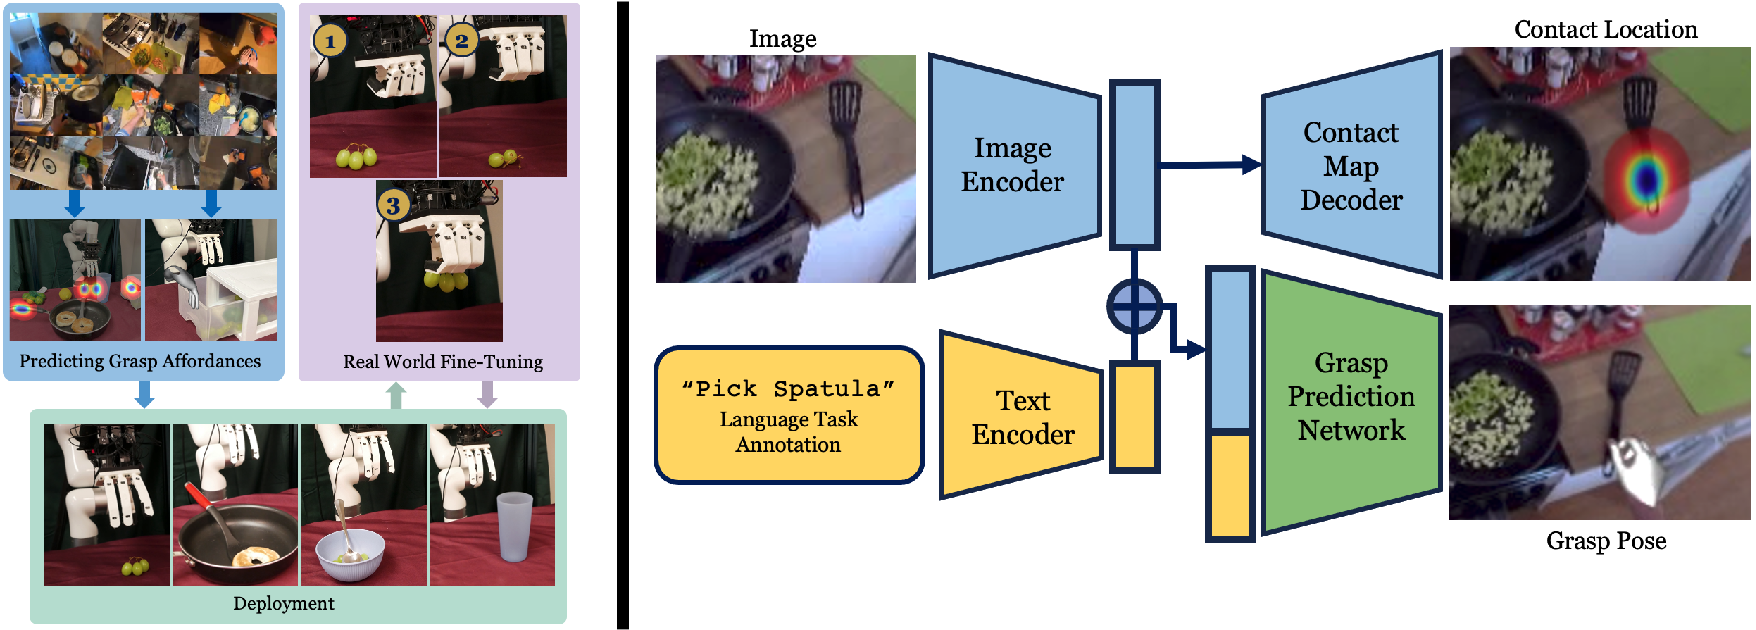
\includegraphics[width=\linewidth]{figs/method_overview.pdf}
\vspace{-0.2in}
  \caption{\small \textbf{Left:}  \ours consists of two phases: an affordance model that predicts grasp parameters followed by online fine-tuning with CEM. \textbf{Right:} Our affordance prediction setup predicts grasp location and pose.}
 \label{fig:aff_method}
 \vspace{-0.15in}
\end{figure}

The goal of \ours is to learn useful, dexterous manipulation in the real world that can generalize to many objects and scenarios.  \ours learns in the real-world and fine-tunes robot hand-to-object interaction in the real world using only a few samples. However, without any priors on what is useful behavior, the robot will explore the action space inefficiently. Especially with a high-dimensional robotic hand, we need a strong prior to effectively explore the real world. We thus train an affordance model on human videos that leverages human behavior to learn what are reasonable behaviors the robot should perform.  

\section{Learning grasping affordances}
\begin{figure}[t]
\centering
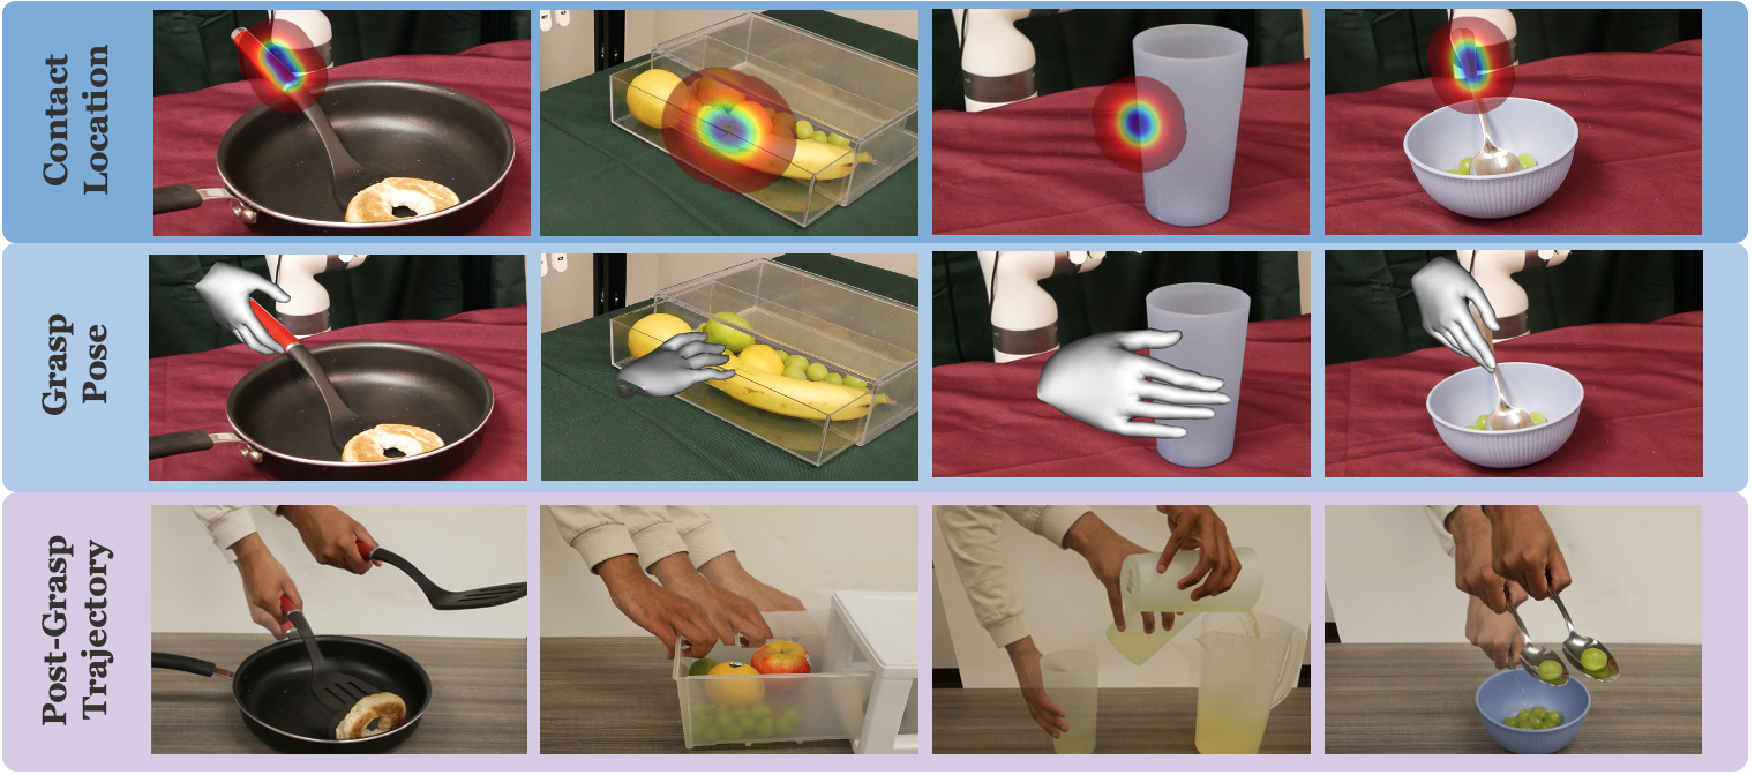
\includegraphics[width=\linewidth]{figs/aff_results.pdf}
\vspace{-0.2in}
  \caption{\small We produce three priors from human videos: the contact location (\textbf{top row}) and grasp pose (\textbf{middle row}) from the affordance prior; the post-grasp trajectory (\textbf{bottom row}) from a human demonstration of the task.}
 \label{fig:aff_results}
 \vspace{-0.15in}
\end{figure}


% \begin{wrapfigure}{l}{0.5\textwidth}
% \vspace{-0.3in}
% \begin{minipage}{\linewidth}
% \begin{algorithm}[H]
% \caption{\small Training affordances for \ours}\label{alg:cap}
% \begin{algorithmic}
% \small
% \REQUIRE Human videos $V_{1:K}$, task descriptions $T_{1:K}$, affordance model $f$. Human detection $f_\text{human}$ \citep{FrankMocap_2021_ICCV}. 

% \end{algorithmic}
% \label{algo:affordance}

% \end{algorithm}
% \end{minipage}
% \end{wrapfigure}


To learn from dexterous interaction in a sample efficient way, we use human hand motion as a prior for robot hand motion. We aim to answer the following: (1) What useful, actionable information can we extract from the human videos? (2) How can human motion be translated to the robot embodiment to guide the robot? In internet videos, humans frequently interact with a wide variety of objects. This data is especially useful in learning object affordances. Furthermore, one of the major obstacles in manipulating objects with few samples is accurately grasping the object. A model that can perform a strong grasp must learn \textit{where} and \textit{how} to grasp. Additionally, the task objective is important in determining object affordances--humans often grasp objects in different ways depending on their goal. Therefore, we extract three pieces of information from human videos: the grasp location, the human grasp pose, and the task.

Given a video clip $V = \{ v_1, v_2, \dots, v_T \} $, the first frame $v_t$ where the hand touches the object is found using a pre-trained, off-the-shelf hand-object detection model \cite{100doh}. Similar to previous approaches \cite{bahl2023affordances, hap, hoi, hotspots}, a set of contact points are extracted to fit a Gaussian Mixture Model (GMM) with centers $\mu = \{ \mu_1, \mu_2, \dots, \mu_k \}$.  Detic \cite{detic} is used to obtain a cropped image $v_1'$ containing just the object in the initial frame $v_1$ to condition the model. We use Frankmocap \cite{FrankMocap_2021_ICCV} to extract the hand grasp pose $P$ in the contact frame $v_t$ as MANO parameters. We also obtain the wrist orientation $\theta_\text{wrist}$ in the camera frame. This guides our prior to output wrist rotations and hand joint angles that produce a stable grasp. Finally, we acquire a text description $T$ describing the action occurring in $V$.

We extract affordances from three large-scale, egocentric datasets: Ego4D \cite{ego4d} for its large scale and the variety of different scenarios depicted, HOI4D \cite{hoi4d} for high-quality human-object interactions, and EPIC Kitchens \cite{EPICKITCHENS} for its focus on kitchen tasks similar to our robot's. We learn a task-conditioned affordance model $f$ that produces $(\hat{\mu}, \hat{\theta}_\text{wrist}, \hat{P}) = f(v_1', T)$. We predict $\hat{\mu}$ in similar fashion to \cite{bahl2023affordances}. First, we use a pre-trained visual model \cite{r3m} to encode $v_1'$ into a latent vector $z_v$. Then we pass $z_v$ through a set of deconvolutional layers to get a heatmap over $v_1'$ and use a spatial softmax to estimate $\hat{\mu}$.

To determine $\hat{\theta}_\text{wrist}$ and $\hat{P}$, we use $z_v$ and an embedding of the text description $z_T = g(T)$, where $g$ is the CLIP text encoder \cite{Clip}. Because transformers have seen success in encoding various multiple modes of input, we use a transformer encoder $\mathcal{T}$ to predict $\hat{\theta}_\text{wrist}, \hat{P} = \mathcal{T}(z_v, z_T)$. Overall, we train our model to optimize
\begin{align}
    \mathcal{L} = \lambda_\mu || \mu - \hat{\mu} ||_2 + \lambda_\theta || \theta_\text{wrist} - \hat{\theta}_\text{wrist} ||_2 + \lambda_P || P - \hat{P} ||_2
\end{align}


At test time, we generate a crop of the object using Segment-Anything \cite{kirillov2023segment} and give our model a task description. The model generates contact points on the object, and we take the average as our contact point. Using a depth camera, we can determine the 3D contact point to navigate to. While the model outputs MANO parameters \cite{MANO:SIGGRAPHASIA:2017} that are designed to describe human hand joints, we retarget these values to produce similar grasping poses on our robot hand in a similar manner to previous approaches \cite{handa2020dexpilot, sivakumar2022robotic}. For more details, we refer readers to the appendix. In addition to the affordance model $f$, we collect one demo of the human doing the robot task (Figure~\ref{fig:aff_results}). This demo is used as a prior on the post-grasp trajectory.  We extract the task-specific wrist trajectory after the grasp using \cite{FrankMocap_2021_ICCV}. In the fine-tuning stage, we initialize the post-grasp trajectory with this human demonstration. Once we have this prior, how can the robot \textit{improve} upon it? 


\section{Fine-tuning via Interaction}

\begin{wrapfigure}{l}{0.55\textwidth}
\vspace{-0.3in}
\begin{minipage}{\linewidth}
\begin{algorithm}[H]
\caption{\small Fine-Tuning Procedure for \ours}\label{alg:cap}
\begin{algorithmic}
\small
\REQUIRE Task-conditioned affordance model $f$, task description $T$, post-grasp trajectory $\tau$, residual policy $\pi$. $E$ number of elites, $M$ number of warm-up episodes, $N$ total iterations. 

\FOR{$k = 1 \dots N$}
    \STATE $I_{k, 0} \gets $ initial image
    \STATE $\xi_k \gets f(I_{k, 0}, T)$
    \STATE $\epsilon_k = \pi(I_{k, 0}, \xi_k)$
    \STATE Execute grasp from $\xi_k + \epsilon_k$, then trajectory $\tau$
    \STATE Collect reward $R_k$; reset environment

    \IF{$k > M$}
        \STATE Order traj indices $i_0, i_1, \dots, i_k$ based on rewards
        \STATE $E \gets \{ \epsilon_{i_0}, \epsilon_{i_1}, \dots, \epsilon_{i_E} \} $
        \STATE Fit $\pi(.)$ as a VAE to $E$
    \ENDIF
\ENDFOR

\end{algorithmic}
\label{algo:finetune}

\end{algorithm}
\end{minipage}
\end{wrapfigure}


The affordance prior allows the robot to narrow down its learning behavior to a small subset of all possible behaviors. However, these affordances are not perfect and the robot will oftentimes still not complete the task.  This is partially due to morphology differences between the human and robot hands, inaccurate detections of the human hands, or differences in the task setup. In order to improve upon this, we practice in an online fashion to optimize the learned skills. 

Let the grasp location, wrist rotation and grasp pose, as well as the trajectory from our affordance prior be $\xi$. During training we sample noise $\epsilon \sim \mathcal{D}$ where $\mathcal{D}$ is initialized to $\mathcal{N}(0, \sigma^2)$ (for a small $\sigma$). We rollout a trajectory parameterized by $\xi + \epsilon$. We collect $R_i$, the reward for each $\xi_i = f(v_i) + \epsilon_i$ where $v_i$ is the image.  After an initial number of $M$ warmup episodes, we rank the rollouts based on $R_i$ and extract sampled noise from the elite trajectories $\{ \epsilon_{i_1}, \epsilon_{i_2}, \dots, \epsilon_{i_k} \}$. We fit $\mathcal{D}$ to the elite trajectories to improve the sampled noise. 

At test time, we could take the mean values of the top $N$ trajectories for the rollout policy.  However, this does not account for the appearance of different objects, previously unseen object configurations, or other properties in the environment. To account for this, we train a VAE \cite{SohnNIPS2015, rezende2014stochastic, rezende2014vae, kingma2013vae} to output residuals $\delta_j$ conditioned on an encoding of the initial image $\phi(I_{j, 0})$ and affordance model outputs $\xi_j$ from the top ten trajectories. We train an encoder $q(z | \delta_j, c_j)$ where $c_j = (\phi(I_{j, 0}), \xi_j)$, as well as a decoder $p(\delta_j | z, c_j)$. At test time, our residual policy $\pi (I_0, \xi)$ samples $z \sim \mathcal{N}(\mathbf{0}, \mathbf{I})$ and predicts $\hat{\delta} = p(z, (I_0, \xi))$. Then we rollout the trajectory determined by the parameters $\xi + \hat{\delta}$. We provide more details in the Appendix. 

\chapter{Experimental Setup}
\label{sec:setup}

\begin{figure}[H]
\centering
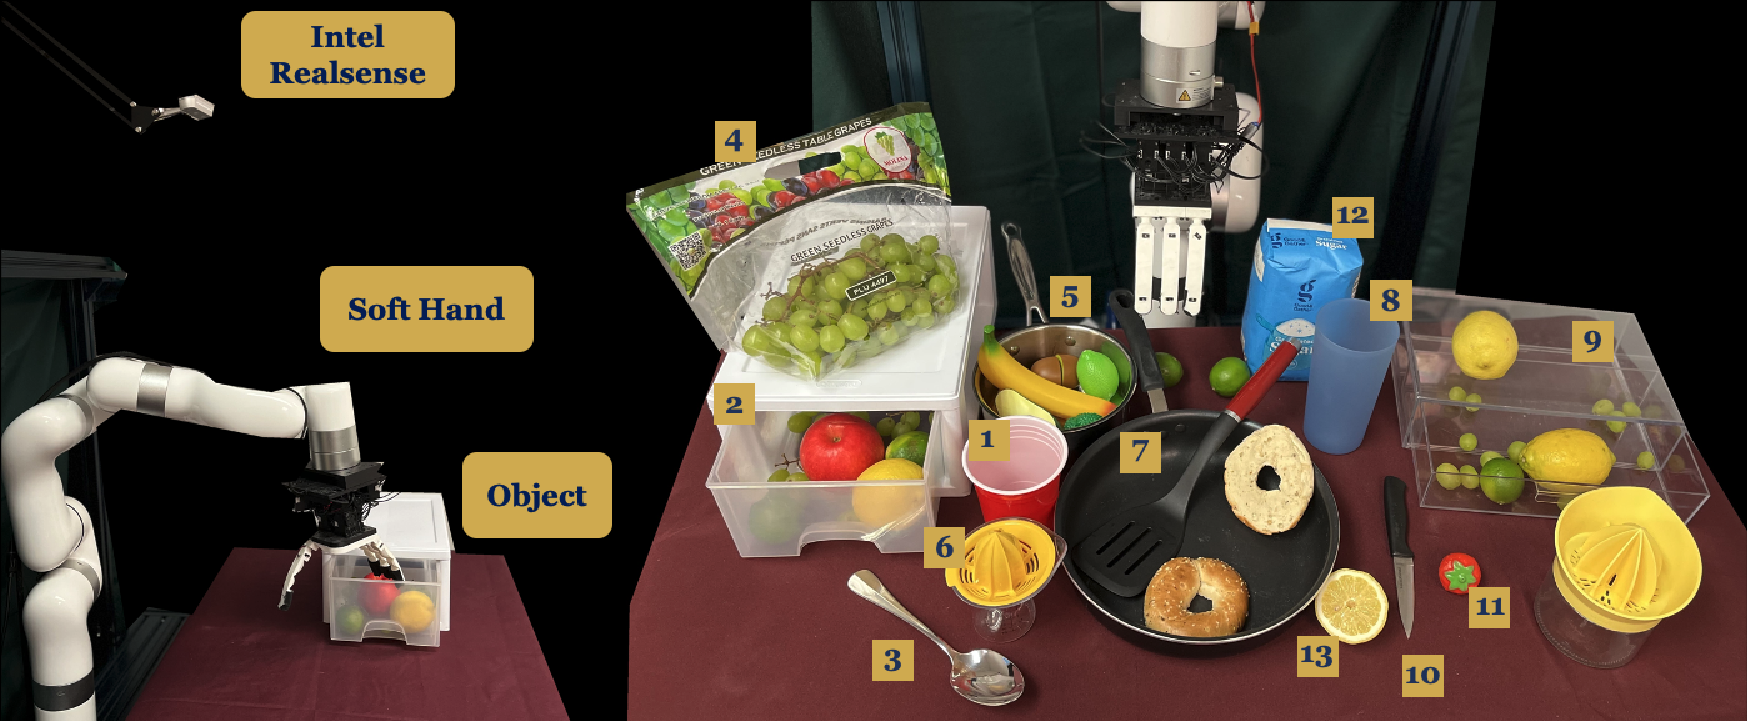
\includegraphics[width=\linewidth]{figs/workspace.pdf}
\vspace{-0.2in}
  \caption{\small \textbf{Left}: Workspace Setup. We place an Intel RealSense camera above the robot to maintain an egocentric viewpoint, consistent with the affordance model's training data. \textbf{Right}: Thirteen objects used in our experiments.}
 \label{fig:workspace}
 \vspace{-0.15in}
\end{figure}

\section{Task Setup} We introduce 9 tabletop tasks: \textit{Pick Cup}, \textit{Pour Cup}, \textit{Open Drawer}, \textit{Pick Spoon}, \textit{Scoop Grape}, \textit{Stir Spoon}, \textit{Pick Grape}, \textit{Flip Bagel}, and \textit{Squeeze Lemon}. For all tasks, we randomize the position of the object on the table, as well as use train and test objects with different shapes and appearances to test for generalization. See Figure~\ref{fig:workspace} for a depiction of the robot's workspace and the objects we use in our experiments.

We define the success criteria in each of our 9 tasks as follows:

\begin{itemize}
    \item Pick Cup: Cup must leave table surface and stay grasped throughout trial.
    \item Pour Cup: Cup must be grasped throughout trial and also rotate so that the top of the cup is at a lower height than the base.
    \item Open Drawer: Drawer is initially slightly open so that it can be grasped. By the end of the rollout, the drawer should be at least 1 centimeter more open than it was at the beginning.
    \item Pick Spoon: The spoon must not be in contact with the table at the end of the trial.
    \item Stir Spoon: The spoon base must rotate around the jar/pot at least 180 degrees while grasped.
    \item Scoop Grape: The spoon must have a grape at the end of the trial while being held by the soft hand.
    \item Pick Grape: All grapes must be held by the hand above the table surface. In particular, if any single grape falls due to a weak stem, this is considered a failure.
    \item Flip Bagel: The side of the bagel that is facing up at the end of the trial should be opposite the side facing up at the beginning.
    \item Squeeze Lemon: The lemon should be grasped securely on top of the juicer.
\end{itemize}

\section{Online Fine-Tuning Setup}

To achieve real-world learning with the soft robot hand, we pretrain an internet affordance model as a prior for robot behavior.  As explained in Section \ref{sec:method}, we train one language-conditioned model on all data.  At test time, we use this as initialization for our real-world fine-tuning. The fine-tuning is done purely in the real world.  An operator runs 10 warmup episodes of CEM, followed by 20 episodes that continually update the noise distribution, improving the policy. We train a residual VAE policy that trains on the top ten CEM rollouts to predict the noise given the image and affordance outputs. Over all our experiments, we collect data for several thousands of rollouts for over 100 hours of real world data collection.

\section{Datasets and Affordance Model Parameters}

We use data from Ego4D \cite{ego4d}, EpicKitchens-100 \cite{EPICKITCHENS}, and HOI4D \cite{hoi4d}.  After filtering for clips of sufficient length, clips that involve grasping objects with the right hand, and clips that have language annotations, we used 64666 clips from Ego4D, 9144 clips from EpicKitchens, and 2707 clips from HOI4D. In total, we use a dataset of 76517 samples for training our model.

For our contact location model, we use the visual encoder from \cite{r3m} to encode the image as a 512-dimensional vector. We use the spatial features of the encoder to upsample the latent before applying a spatial softmax to return the contact heatmap. This consists of three deconvolutional layers with 512, 256, and 64 channels in that order.

To predict wrist rotation and grasp pose, we use the language encoder from \cite{Clip} to compress the language instruction to a 512-dimensional vector. We concatenate the visual and language latents and pass it through a transformer with eight heads and six self-attention layers. We pass the result of the transformer through an MLP with hidden size 576, and predict a vector of size 48: the first 3 dimensions are the axis-angle rotations; the last 45 dimensions are the joint angles of the hand. These correspond to the parameters output by Frankmocap \cite{FrankMocap_2021_ICCV}, which we used to get ground truth hand pose in all the datasets.

We jointly optimize the L2 loss of the contact location $\mu$, the wrist rotation $\theta_\text{wrist}$ and grasp pose $P$. The weights we used for the losses are $\lambda_\mu = 1.0, \lambda_\theta = 0.1, \lambda_P = 0.1$. We train for 70 epochs with an initial learning rate of 0.0002, and a batch size of 224. We used the Adam optimizer \cite{kingma2014adam} with cosine learning rate scheduler. We trained on a single NVIDIA RTX A6000 with 48GB RAM.

\section{Hardware Setup}

We use a 6-DOF UFactory xArm6 robot arm for all our experiments. We attach it to a 16-DOF Soft Hand using a custom, 3D-printed base. We use a single, egocentric RGBD camera in order to capture the 3D location of the object in the camera frame. We calibrate the camera so that the predictions of the affordance model can be converted to and executed in the robot frame. The flexibility of the robot hand also makes it robust to collisions with objects or unexpected contact with the environment. 

\section{Safety} 

In our fine-tuning experiments, there is a particular focus on the safety of the robot system and the environment. The soft hand allows the policy to perform high-contact manipulation tasks without breaking because of its compliance. Our method takes advantage of the compliance as it performs thousands of iterations in the real world.

While the end-effector is soft, the arm is not. Because it is susceptible to damage when colliding with the environment, we constrain the arm's velocity and ensure that the arm stays above the tabletop. The rollout will be terminated if the arm's dynamics controller senses that the arm collided aggressively with the environment.
 

\chapter{Results}
\label{sec:results}

We performs a variety of experiments to answer the following questions:  1) How good is our affordance model? 2) How well can \ours learn and improve in the real world? 3) How can the experience collected by \ours be distilled into a policy? 4) How can \ours be used for complex, soft object manipulation? We investigate the role of the affordance model and real-world fine-tuning in Table~\ref{tab:main} and Figure~\ref{fig:graph_main}. Then we perform a series of ablations in Table~\ref{tab:abl}.

\begin{table}[t]
    \centering
    \resizebox{\linewidth}{!}
    {%
        \begin{tabular}{lcccccccccccccccc}
        \toprule
        Method & \multicolumn{2}{c}{Pick cup} & \multicolumn{2}{c}{Pour cup} & \multicolumn{2}{c}{Open drawer} & \multicolumn{2}{c}{Pick spoon} & \multicolumn{2}{c}{Scoop Grape} & \multicolumn{2}{c}{Stir Spoon} & \\ 
        & train & test & train & test & train & test & train & test & train & test & train & test \\
        \midrule
        \
        \textbf{\texttt{Real-World Only}} & 0.0 & 0.1 & 0.2 & 0.1 & 0.1 & 0.0 & 0.7 & 0.3 & 0.0 & 0.0 & 0.3 & 0.0 \\ 
        \textbf{\texttt{Affordance Model Only}} & \multicolumn{2}{c}{0.1} & \multicolumn{2}{c}{0.4} & \multicolumn{2}{c}{\textbf{0.5}} & \multicolumn{2}{c}{0.5} & \multicolumn{2}{c}{0.0} & \multicolumn{2}{c}{0.3}\\ 
        
        \midrule
        \textbf{\texttt{\ours}} & \textbf{0.8} & \textbf{0.8} & \textbf{0.8} & \textbf{0.9} & \textbf{0.5} & \textbf{0.4} & \textbf{0.8} & \textbf{0.6} & \textbf{0.7} & \textbf{0.3} & \textbf{0.8} & \textbf{0.5}\\
        %%\textbf{\texttt{\ours First Iteration}} & 0.0 & 0.0 & 0.1 & 0.0 & 0.4 & 0.2 & 0.6 & 0.5 & 0.1 & 0.2 & 0.5 & 0.4\\ 
        \bottomrule
        \end{tabular}
    }
    \vspace{0.05in}
    \caption{We present the results of our method as well as compare them to other baselines: Real-world learning without internet priors used as guidance and the affordance model outputs without real-world learning.  Together, our method is able to better complete these tasks.}
    \label{tab:main}
\end{table}



\begin{figure}[t]
\centering
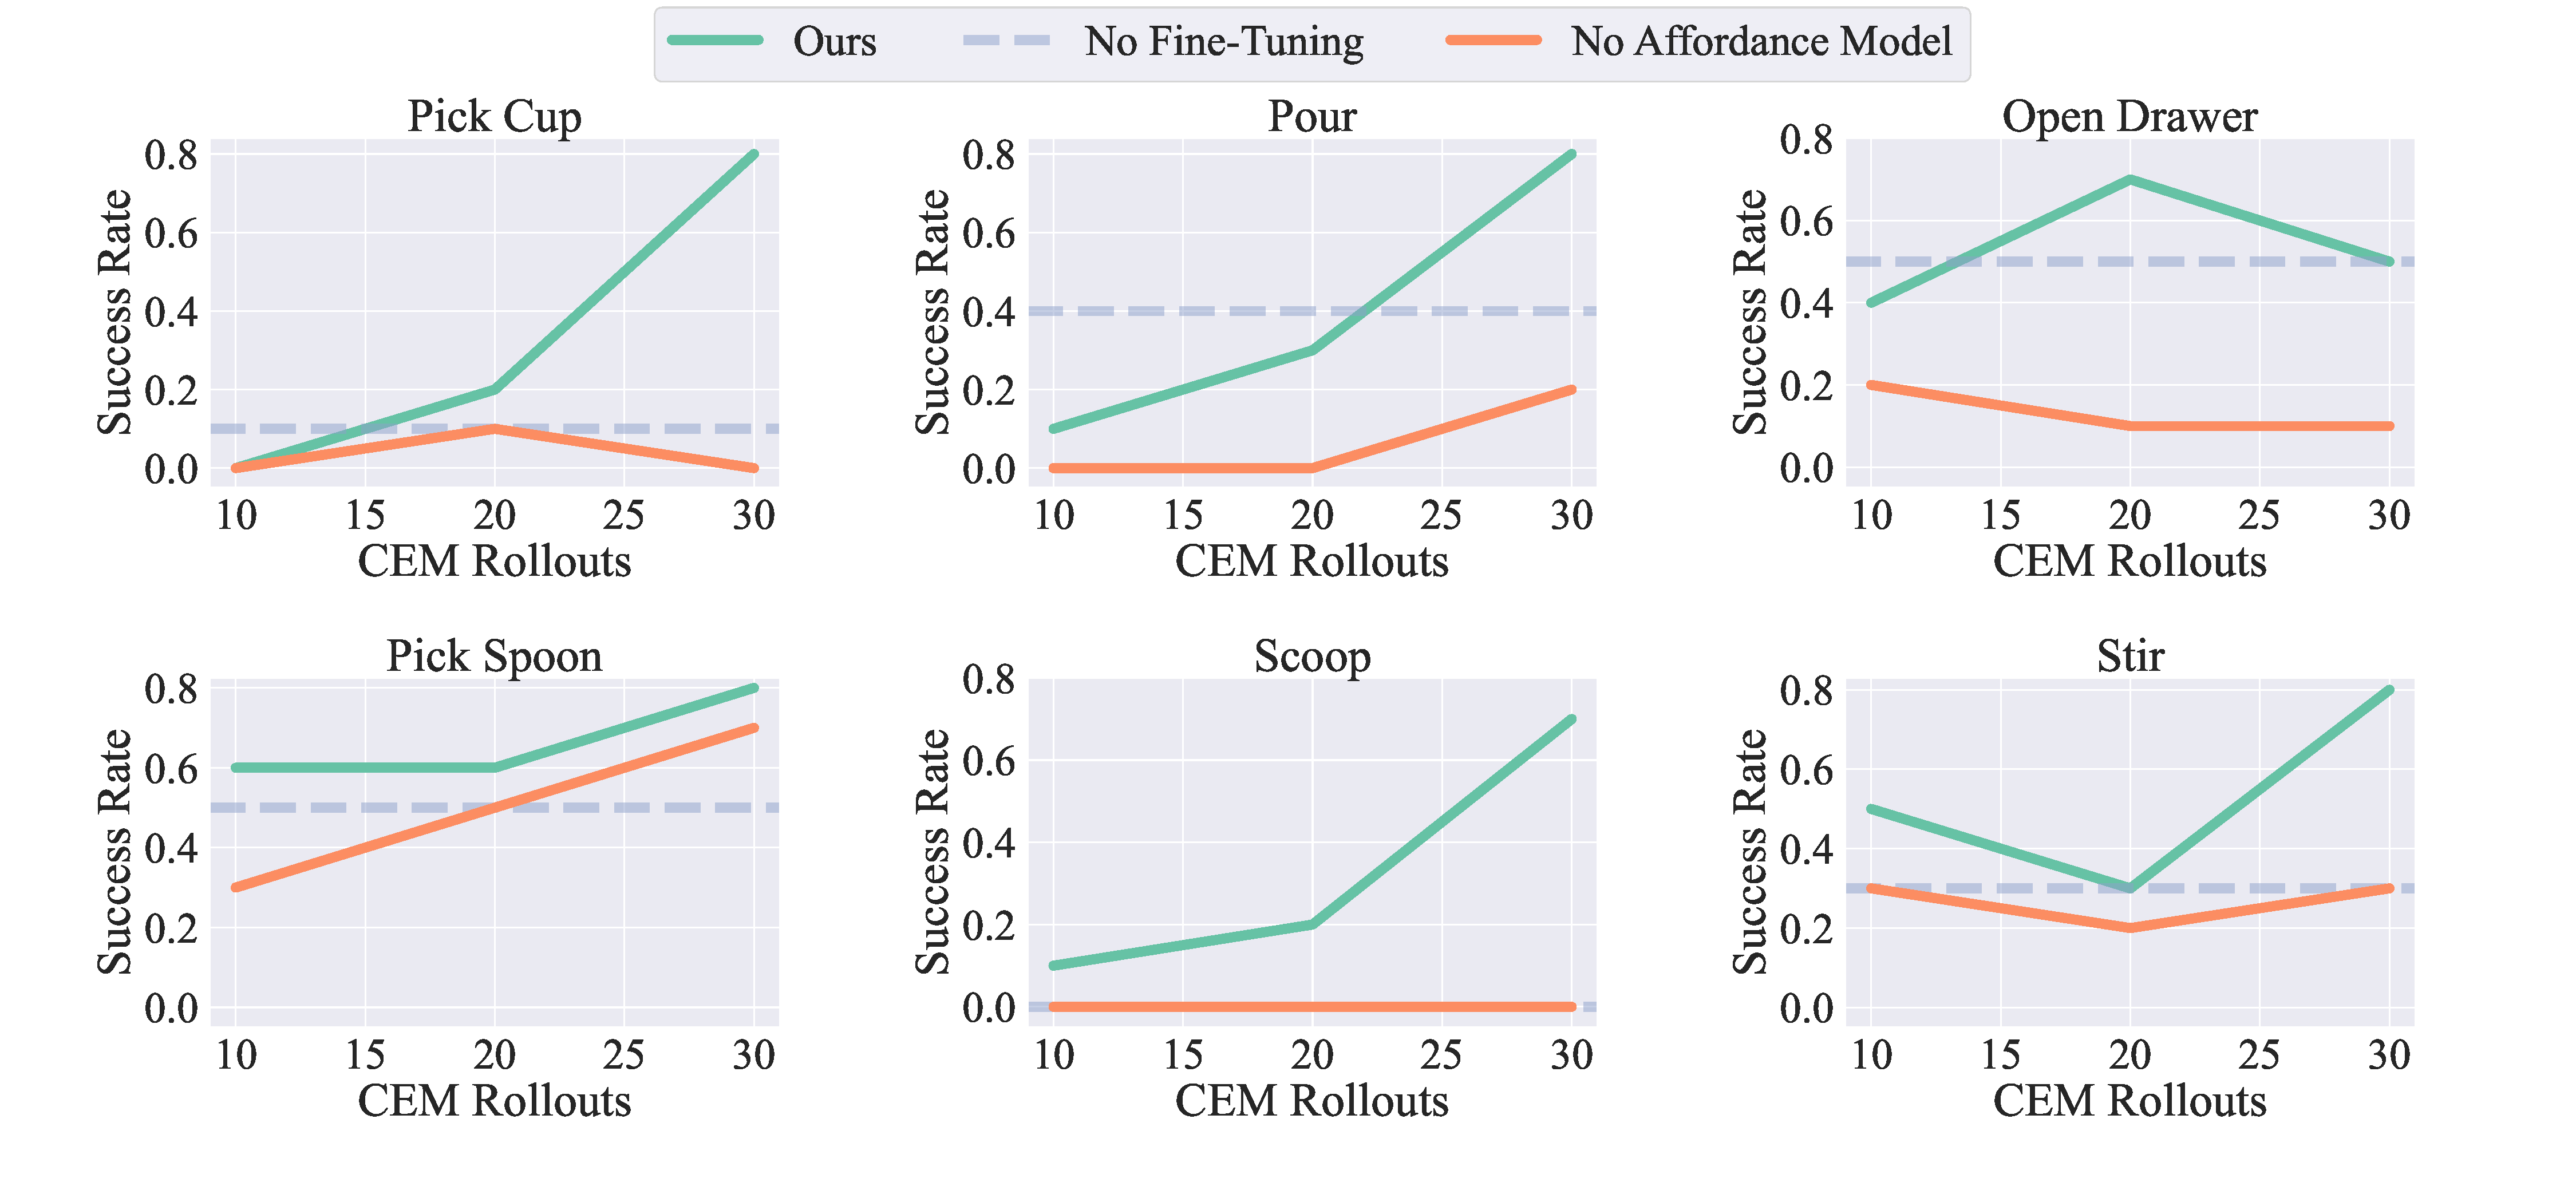
\includegraphics[width=\linewidth]{figs/graphs_main.pdf}
\vspace{-0.25in}
  \caption{\small Improvement results for 6 tasks: pick cup, pour, open drawer, pick spoon, scoop, and stir. We see a steady improvement in our method as more CEM episodes are collected.
}
 \label{fig:graph_main}
 \vspace{0.1in}
\end{figure}


\section{Effect of affordance prior} 
The human affordance model predicted three items: the contact location, the wrist grasp rotation, and and the hand joint pose. In the Real-World Only model, we use a few heuristics in place of each item in the affordance prior and proceed with fine-tuning. For contact location, we detect the object in the scene using a popular object detection model \cite{kirillov2023segment} and let the contact location prior be the center of the bounding box. For the wrist rotation, use a generic rotation with the pal of the hand facing downward. Finally, for the hand joint angles, we fix a half-closed hand as the grasp pose prior.  

With these heuristics, the robot has difficulty finding stable grasps consistently across a range of tasks. While the robot is able to navigate to the object, the main obstacle was finding the correct rotation angle for the hand. Hand rotation is very important for many tool manipulation tasks because it requires not only picking the tool but also grasping in a stable manner. While the soft hand shows decent success in grasping a spoon (where the grasp rotation from the heuristic is close to the correct grasp rotation) it is not able to perform well in tasks that require other wrist rotations.

It is possible that with more exploration the Real-World Only model would be able to catch up with \ours. However, we believe that these results indicate that the human affordance model reduces the number of fine-tuning episodes necessary in the real world.

\section{Zero-shot model execution} 
We explore the zero-shot performance of our prior with the Affordance Only model.  Without applying any online fine-tuning to our affordance model, we rollout the trajectory parameterized by the prior.  While our model performs decent on simpler tasks, the model struggles on tasks like stir and scoop that require strong, power grasps (shown in Table~\ref{tab:main}). In these tasks, the spoon collides with other objects, so fine-tuning the prior to hold the back of the spoon is important in maintaining a reliable grip throughout the post-grasp motion. Because \ours incorporates real-world experience with the prior, it is able to sample contact locations and grasp rotations that can better execute the task. 

One observation we found is that our zero-shot model sometimes performs better than the residual model trained on the first ten CEM iterations. This is due to \ours optimizing the grasp parameters only after ten iterations. Our first residual model learns only from random noise, explaining why our zero-shot performance can be stronger than \ours after few iterations of fine-tuning.


\begin{figure}[t]
\centering
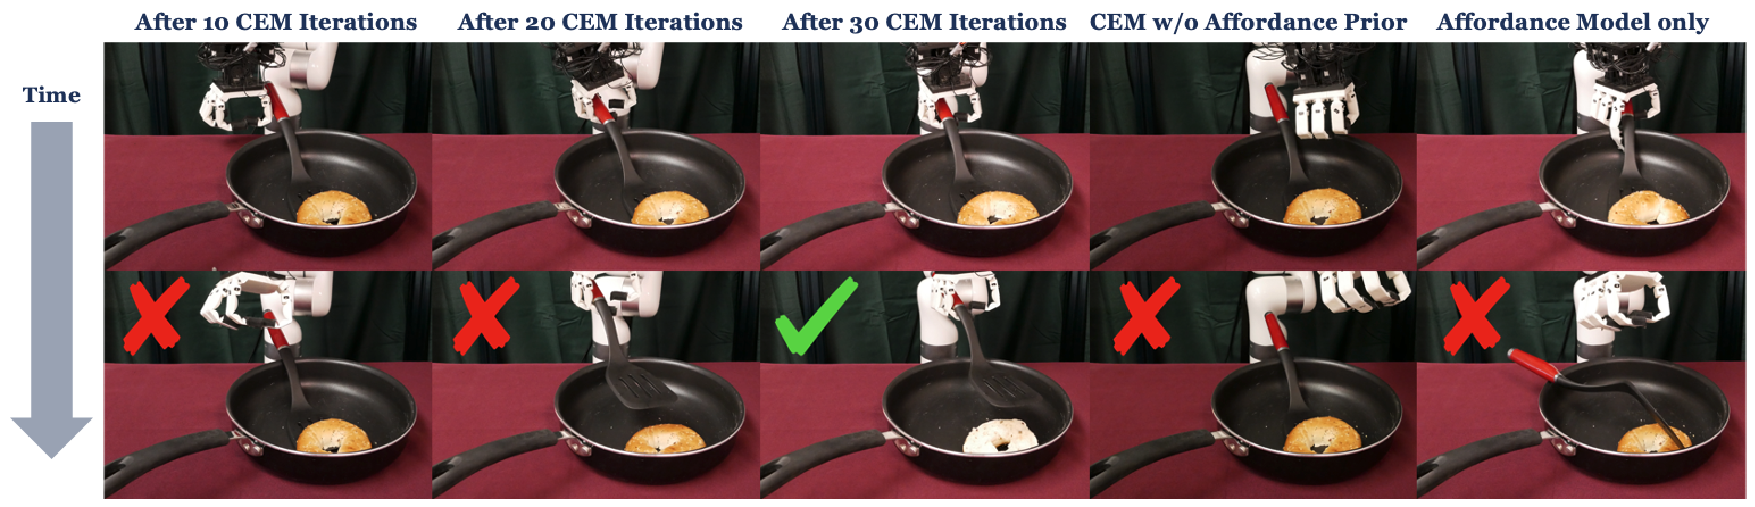
\includegraphics[width=\linewidth]{figs/qual_results.pdf}
\vspace{-0.2in}
  \caption{\small Qualitative results showing the finetuning procedure for \ours.  The model learns to hold the spatula and flip the bagel after 30 CEM iterations. }
 \label{fig:task_bagel}
 \vspace{-0.15in}
\end{figure}


\section{Human and automated rewards}
Our method queries the operator during the task reset process to assign a continuous score from $0$ to $1$ for the grasp.  Because the reset process requires a human-in-the-loop regardless, this adds little marginal cost for the operator.  But what if we would like these rewards to be calculated autonomously?  

We use the final image collected in the single post-grasp human demonstration from Section \ref{sec:method} as the goal image.  We define the reward to be the negative embedding distance between the final image of the rollout and the goal image with either an R3M \cite{r3m} or a ResNet \cite{resnet} encoder. The model learned from ranking trajectories with R3M reward is competitive with \ours in two of the three tasks we tested on, and performed better than the model that used Resnet18 rewards. Using a third-person camera could potentially improve the rankings because changes in the object will be more apparent. Nevertheless, these results indicate that using a visual reward model can potentially provide reasonable results compared to human rewards.

\begin{table}[t]
    \centering
    \resizebox{0.85\linewidth}{!}
    {%
        \begin{tabular}{lcccccc}
        \toprule
        Method & \multicolumn{2}{c}{Pour Cup} & \multicolumn{2}{c}{Open Drawer} & \multicolumn{2}{c}{Pick Spoon}  \\ 
         &train & test & train & test & train & test\\
        \midrule
        \multicolumn{2}{l}{\textit{Reward Function:}}\vspace{0.0em}\\
        \textbf{\texttt{R3M Reward}} & 0.0 & 0.0 & 0.4 & \textbf{0.5} & 0.5 & 0.4\\ 
        \textbf{\texttt{Resnet18 Imagenet Reward}} & 0.1 & 0.2 & 0.3 & 0.1 & 0.4 & 0.2\\ 
        \midrule
        \multicolumn{2}{l}{\textit{Policy Ablation:}}\vspace{0.0em}\\
        \textbf{\texttt{\ours w/ MLP}} & 0.0 & 0.0 & 0.5 & 0.0 & 0.6 & 0.5\\ 
        \textbf{\texttt{\ours w/ Transformer}} & 0.4 & 0.5 & \textbf{0.6} & 0.1 & 0.4 & 0.5\\  
        \textbf{\texttt{\ours w/ Direct Parameter est.}} & 0.1 & 0.1 & 0.1 & 0.0 & 0.3 & 0.0\\ 
        \midrule
        \textbf{\texttt{\ours }} & \textbf{0.8} & \textbf{0.9} & 0.5 & 0.4 & \textbf{0.8} & \textbf{0.6} \\ 
        \bottomrule
        \end{tabular}
    }
    \vspace{0.05in}
    \caption{Ablations for (1) reward function type, (2) model architecture, and (3) parameter estimation approach.}
    \label{tab:abl}
\end{table}


\section{Model Architecture} We investigate different models and training architectures for the policy trained on the rollouts (Table~\ref{tab:abl}). When we replace the conditional VAE with an MLP that predicts residuals, the model has difficulty learning the grasp rotation to effectively pour a cup. This may be because VAEs can compress multi-modal data more effectively (which is useful for our case as our data includes location, rotation, and joint angles).

Our transformer ablation is an offline method similar to \cite{chen2021decisiontransformer} where in addition to the image and affordance model outputs, we condition on the reward outputs and train a transformer to predict the residual. At test time the maximum reward is queried and the output is used in the rollout. We hypothesize that the reduced performance is because the transformer is a data-hungry architecture. The model may need more real-world data, which can be expensive to collect.

Finally, we train a VAE to directly estimate $\xi$ instead of the residual. This model was unable to effectively distill the information from the affordance prior with neither the diversity of data nor training time allotted. As a result, it often makes predictions that are far from the correct grasp pose. 


\begin{figure}[t]
\vspace{-0.2in}
\begin{center}
    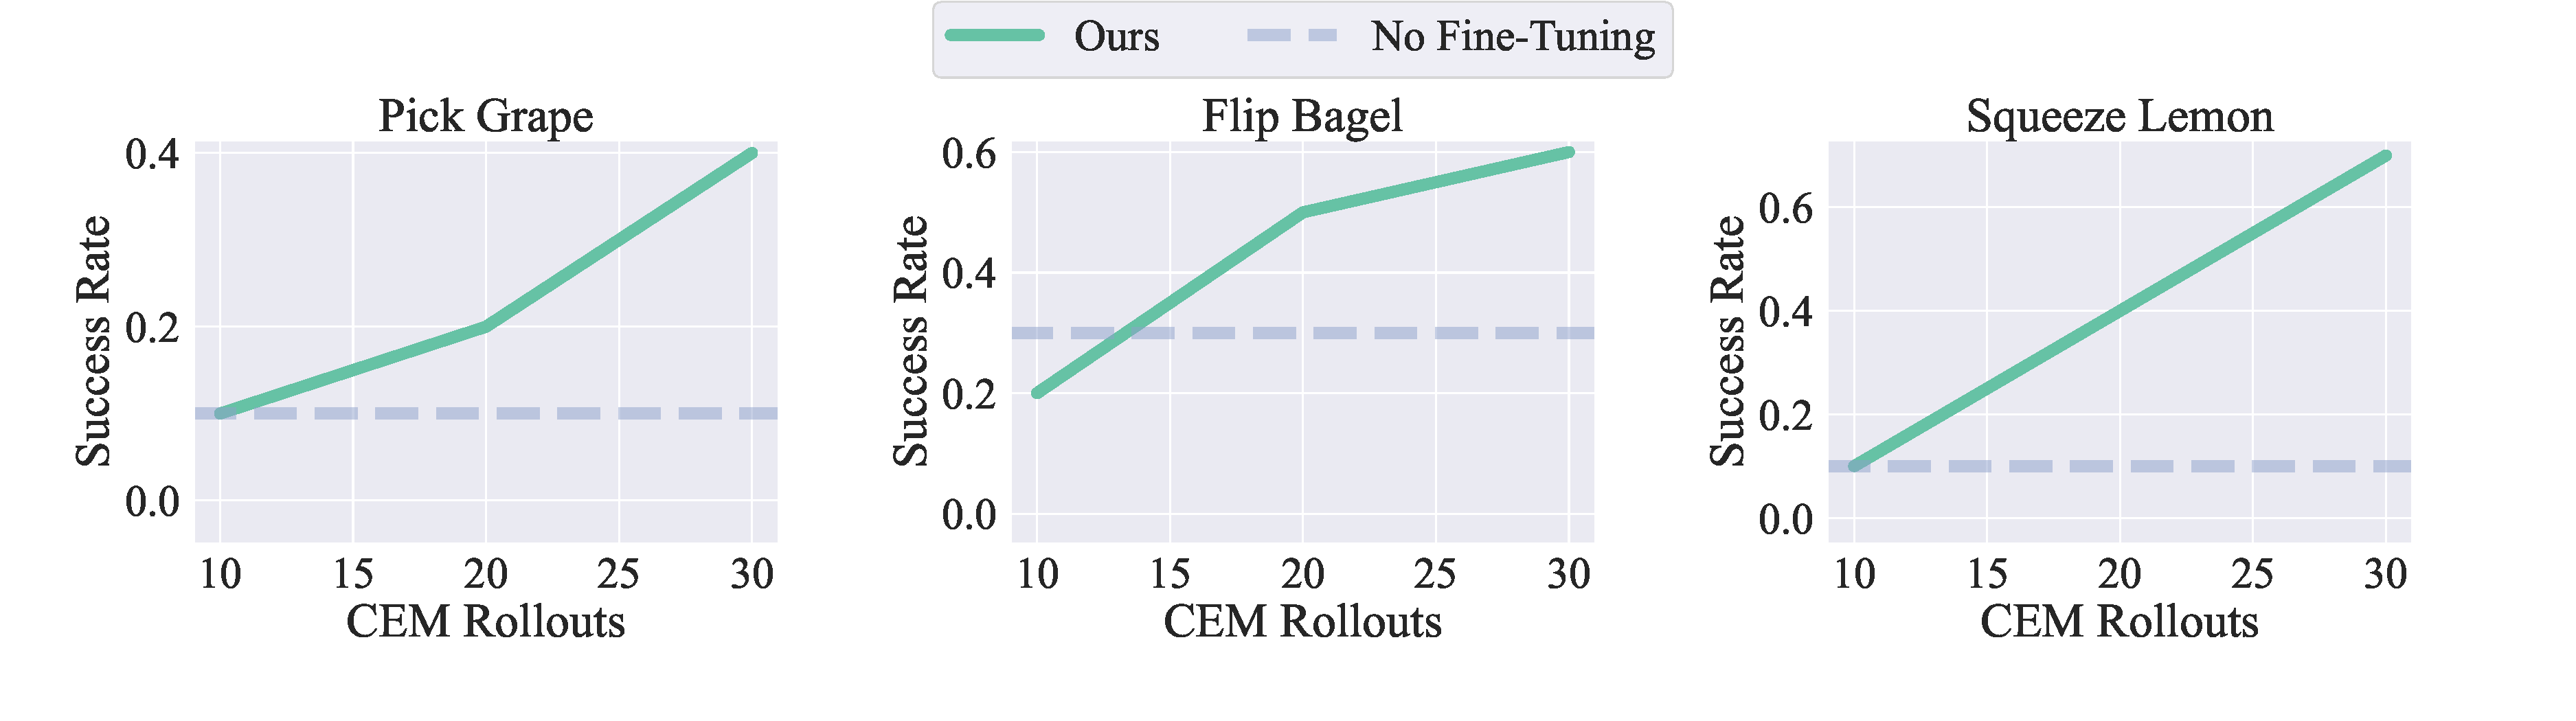
\includegraphics[width=\linewidth]{figs/graphs_difficult.pdf}
\end{center}
\vspace{-0.1in}
  \caption{\footnotesize We evaluate \ours on three additional difficult manipulation tasks. }
 \label{fig:graph_difficult}
 \vspace{-0.15in}
\end{figure}


\section{Performance on complex tasks and soft objects} 
We investigate the performance of \ours on more challenging tasks, which involve grasping or manipulating food. Tasks involving soft objects cannot be simulated accurately, so sim2real methods may have difficulty performing these tasks in the real world. Our method does not have that challenge in this setting and \ours is able to perform reasonably well after on these tasks.

Of the three tasks, our method has the most difficulty with the Pick Grape task. This is because grapes are small and require the fingers to curl fully to maintain a stable grasp. A limitation of our hand is that the range of MCP joint does not allow the fingertips to touch its palm, and as a result it has difficulty in consistently picking small objects.

\chapter{Discussion and Limitations}
\label{sec:discussion}

In this thesis, we investigate how to learn dexterous manipulation in complex setups. \ours aims to learn directly in the real world. In order to real world fine-tuning, we build an \textit{affordance} prior learned from human videos. We are able to efficiently practice and improve in the real world via our online fine-tuning approach, as well as the use of a soft anthropomorphic hand, performing a variety of tasks (involving both rigid and soft objects).

However, there are some limitations to our work.  While we are able to learn policies for the high-dimensional robot hand, the grasps learned are not multi-modal and do not capture all of the different grasps humans are able to perform.  In particular, we find that the predicted hand poses are all power grasps, which is used even in situations where other grasps might be more appropriate (such as a pinch grasp when picking a grape). We believe that this is mainly caused by noisy hand detections. As these detection models improve, we hope to be able to learn a more diverse set of hand grasps. 

Second, during finetuning, we require resets require human input and intervention. This limits the amount of real-world learning we can do, as the human has to be constantly in the loop to reset the objects. Other works \cite{chen2022single, guptaYuZhaoKumar2021reset} introduce paradigms that might potentially be useful in helping scale our method for more fine-tuning iterations.

Third, the arm has additional physical limitations. While the DASH hand is soft like the human hand, the robot arm is rigid. As a result, the robot cannot mimic \textit{every} grasp humans make. For example, any underhand grasp that involves sliding the hand underneath an object is not possible with this setup because the arm would collide with the table. A soft arm, in addition to a soft hand, would enable a wider range of human-like grasps.

Finally, the soft hand's fingers do not curl fully. The soft hand's fingers have a tradeoff between the strength and range of motion. The version of the soft hand used for the experiments in this thesis has high strength, which is useful to pick large, heavier objects. However, this makes grasping smaller objects, such as individual grapes, more difficult. A hand that can have the best of both worlds would facilitate a larger variety of tasks and is a potential area for future research.

\chapter*{Bibliography}
\addcontentsline{toc}{chapter}{Bibliography}

\vspace{-25mm}
This bibliography contains \total{citenum} references.
\vspace{10mm}

\printbibliography[heading=none]

\end{document}

%%% Local Variables:
%%% coding: utf-8
%%% mode: latex
%%% TeX-engine: xetex
%%% End:
